\documentclass[11pt,a4paper]{article}

% Fonts: TeX Gyre Pagella with matching math (Palatino-style, conventional academic look)
% Loaded by file name because the TeX Live OpenType files are not registered
% with the OS font database on most Linux distributions.
\usepackage{fontspec}
\usepackage{unicode-math}
\setmainfont{texgyrepagella}[
  Extension      = .otf,
  UprightFont    = *-regular,
  BoldFont       = *-bold,
  ItalicFont     = *-italic,
  BoldItalicFont = *-bolditalic,
]
\setmathfont{texgyrepagella-math.otf}
\frenchspacing

% Page layout
\usepackage[margin=1in]{geometry}

% Math
\usepackage{amsmath,amsthm}

% Tables
\usepackage{booktabs}
\usepackage{array}

% Figures
\usepackage{graphicx}
\usepackage{float}
\usepackage[section]{placeins}

% Captions: small, bold-labelled
\usepackage{caption}
\captionsetup{font=small,labelfont=bf}

% Lists
\usepackage{enumitem}

% Prevent orphaned headings
\usepackage{needspace}

% Paragraph formatting
\usepackage{parskip}

% Typographic refinement (better letter spacing, hyphenation, line breaks)
\usepackage{microtype}

% Tighter bibliography spacing
\usepackage{etoolbox}
\AtBeginEnvironment{thebibliography}{\setlength{\itemsep}{4pt plus 0.5pt}\setlength{\parsep}{0pt}}

% Colour expressions for hyperref
\usepackage{xcolor}

% Hyperlinks (subtle dark-blue, all-clickable)
\usepackage{hyperref}
\hypersetup{
  colorlinks=true,
  allcolors=blue!50!black,
  pdfauthor={K.R. Ryan},
  pdftitle={The Geometric Siphon: Emergent Capital Reallocation in Concentrated Liquidity Portfolios}
}

% Running header on pages 2+
\usepackage{fancyhdr}
\pagestyle{fancy}
\fancyhf{}
\fancyhead[L]{\small\itshape K.R.\ Ryan}
\fancyhead[R]{\small\itshape The Geometric Siphon}
\fancyfoot[C]{\thepage}
\renewcommand{\headrulewidth}{0.4pt}
% Title page (page 1) suppresses the running header
\fancypagestyle{plain}{%
  \fancyhf{}%
  \fancyfoot[C]{\thepage}%
  \renewcommand{\headrulewidth}{0pt}%
}

% Theorem environments
\newtheorem{theorem}{Theorem}
\newtheorem*{corollary}{Corollary}

% No paragraph indent, space between paragraphs (match Paper II)
\setlength{\parindent}{0pt}
\setlength{\parskip}{6pt plus 2pt minus 1pt}

\title{The Geometric Siphon: Emergent Capital Reallocation in Concentrated Liquidity Portfolios}

\begin{document}
\thispagestyle{plain}

\begin{center}
{\LARGE\bfseries The Geometric Siphon:\\[4pt]
Emergent Capital Reallocation in\\Concentrated Liquidity Portfolios}

\vspace{12pt}
{\large K.R.\ Ryan}\\[4pt]
{\small Independent Researcher}\\[2pt]
{\small \href{mailto:gancor@gancor.xyz}{gancor@gancor.xyz} \quad|\quad ORCID: 0009-0004-6295-7040}

\vspace{8pt}
March 2026

\vspace{6pt}
{\small\textbf{Keywords:} concentrated liquidity, geometric residual, automated market maker,\\
portfolio rebalancing, Uniswap V3, Aerodrome, DeFi mechanism design}
\end{center}

\vspace{8pt}
\hrule
\vspace{12pt}

\begin{abstract}
This paper identifies and formalises the \textbf{Geometric Siphon}, a previously undocumented mechanism in concentrated liquidity (CL) portfolio management. When multiple CL positions share depositor-level token balances and are autonomously rebalanced, the geometric mismatch between consecutive tick ranges produces token residuals that flow through the shared balance, creating capital transfers between independent positions without oracles, governance or additional gas cost.

I derive a closed-form expression for the geometric residual $\Delta R$ from the Uniswap V3 amount equations and prove that $\Delta R = 0$ if and only if the tick range is unchanged. Any range change produces a non-zero residual that follows directly from the CL amount equations. The theorem is verified with a Foundry test suite running against unmodified Uniswap V3 contracts. Range changes produce measurable residuals (2{,}061 USDC in the test scenario), same-range rebalances produce zero ($< 10^{-6}$ USD), and residuals scale linearly with position size ($4\times$ position $\to$ $4\times$ residual, ratio $4.00$).

Empirical analysis of 1{,}380 rebalance events across 39 positions, five depositor groups, two contract versions and seven days on Aerodrome (Base) reveals a two-mechanism structure: \textbf{Stage~1} (geometric creation, ${\sim}5\%$ of events) produces residuals via range changes that feed the shared dust pool; \textbf{Stage~2} (dust pool redistribution, ${\sim}95\%$ of events) redistributes accumulated dust through same-range rebalances governed by the position-to-pool liquidity ratio $V/L$. The overall decomposition $D = \Delta R - S$ holds at $\rho = 0.976$ with median swap price impact of $0.35\%$.

I prove that single-pool positions converge to equal value under repeated rebalancing (Theorem~\ref{thm:convergence}). A $V/L$ sweep experiment confirms this empirically: positions deployed at ratio $1{:}3{:}9$ collapsed to $1.37{:}1{:}1.20$ within 33 events, with the original size ordering reversed. Multi-pool portfolios settle at position-specific equilibria determined by pool depth. Token-level decomposition across ten pools and five depositor groups reveals the \textbf{Connector Rule}. The siphon driver per pool is the token shared with more portfolio positions, and the same pool exhibits different driver tokens depending on the portfolio's topology.

I prove that positions which rebalance without executing a swap ($S = 0$) decay geometrically: $V_K \leq V_0(1 - \alpha_{\min})^K$ where $\alpha_{\min} > 0$ is the minimum residual fraction per rebalance (Theorem~\ref{thm:extinction}). This result follows from the CL amount equations, the $\min()$ constraint in the liquidity-from-amounts function, and the finiteness of the shared dust pool. The theorem is verified with four additional Foundry tests (7/7 total) and validated against the complete lifecycle of a USDC/ZARP position that lost $99.8\%$ of its capital (\$942 $\to$ \$1.59) in 14 zero-swap rebalances over 65 hours.
\end{abstract}

\section{Introduction}\label{sec:introduction}

\subsection{The problem}\label{sec:problem}

Concentrated liquidity, introduced by Uniswap V3 (Adams et~al., 2021), requires active management. Every major CL automation platform --- Gamma Strategies, Arrakis Finance, Beefy CLM --- uses a \textbf{vault-per-pool architecture} in which one vault manages one token pair and leftover tokens from rebalances are reinvested into the same position.

\begin{verbatim}
Vault-per-pool:    dustBalance[vault]              -> per-pool isolation
Position Manager:  dustBalance[depositor][token]   -> cross-pool sharing
\end{verbatim}

Position Manager V6 (PM V6), a CL management contract on Aerodrome (Base), takes a different approach. Leftover tokens sit in \texttt{dustBalance[depositor][token]}, keyed by depositor and token with no pool dimension. Every position under one depositor draws from the same balance. A capital efficiency decision that unintentionally created cross-position capital flow.

\subsection{Discovery}\label{sec:discovery}

On 2 March 2026, routine monitoring revealed a USDC/CHECK position had grown ${\sim}65\%$ whilst a USDC/ODOS position in the same depositor group had shrunk ${\sim}60\%$. They shared no tokens except USDC. CHECK was consuming USDC residuals left behind by ODOS rebalances through the shared dust pool.

The initial assumption was slippage, but on-chain decomposition of 92 rebalance transactions showed that the transfers are driven almost entirely by the geometric mismatch between consecutive tick ranges. I term this the \textbf{Geometric Siphon}.

\subsection{Scope}\label{sec:scope}

\begin{table}[H]
\centering
\begin{tabular}{@{}llrrll@{}}
\toprule
Phase & Period & Positions & Events & Contract & Focus \\
\midrule
1 & 3--5 Mar 2026 & 22 & 738 & PM V6 & Discovery, topology, regime effects \\
2 & 7--9 Mar 2026 & 17 & 642 & PM V7 & Formalisation, equilibrium, Foundry proof \\
\textbf{Total} & \textbf{7 days} & \textbf{39} & \textbf{1{,}380} & --- & --- \\
\bottomrule
\end{tabular}
\end{table}

\subsection{Contributions}\label{sec:contributions}

\begin{enumerate}[leftmargin=*]
    \item \textbf{Closed-form geometric residual.} $D/V$ is derived as a function of old range, new range and current price from the Uniswap V3 amount equations (\S\ref{sec:residual}). The residual is zero if and only if the range is unchanged (Theorem~\ref{thm:residual}).

    \item \textbf{Independent proof.} Foundry tests against unmodified Uniswap V3 contracts confirm the theorem: range changes create residuals, same-range rebalances do not, and residuals scale linearly with position size (\S\ref{sec:foundry}).

    \item \textbf{Two-mechanism structure.} Stage~1 (geometric creation, ${\sim}5\%$ of events) and Stage~2 (dust pool redistribution, ${\sim}95\%$) are identified as distinct processes with different governing variables (\S\ref{sec:two-mechanism}).

    \item \textbf{Equilibrium proof.} Single-pool positions converge to equal value under repeated rebalancing (Theorem~\ref{thm:convergence}, \S\ref{sec:equilibrium}), confirmed empirically with a controlled $V/L$ sweep experiment (\S\ref{sec:vl-sweep}).

    \item \textbf{Connector Rule.} The siphon driver per pool is determined by the token's connectivity in the portfolio graph, not by relative volatility (\S\ref{sec:connector}, \S\ref{sec:predictive}).

    \item \textbf{Simpson's paradox in CL analysis.} $V/L$ and volatility $\sigma$ are complementary predictors that reverse sign when data are aggregated (\S\ref{sec:predictive}).

    \item \textbf{Zero-swap extinction.} Positions that rebalance without swaps decay geometrically (Theorem~\ref{thm:extinction}, \S\ref{sec:extinction}). A USDC/ZARP position provides a complete empirical lifecycle: \$942 $\to$ \$1.59 in 14 zero-swap rebalances (\S\ref{sec:zarp}). Four additional Foundry tests confirm the theorem (\S\ref{sec:foundry}, 7/7 total).
\end{enumerate}

\begin{center}\rule{0.5\linewidth}{0.5pt}\end{center}

\section{Related work}\label{sec:related}

\textbf{Adams et~al.~(2021)} introduced concentrated liquidity in Uniswap V3. \textbf{Milionis et~al.~(2022a)} developed optimal rebalancing strategies for single CL positions. Their framework provides the theoretical basis for the individual rebalances that produce siphon flows, but assumes positions are independent. This paper studies what happens when they are not.

\textbf{Milionis et~al.~(2022b)} introduced LVR (Loss-Versus-Rebalancing) for quantifying AMM costs. Each rebalance incurs LVR as swap slippage. The decomposition in \S\ref{sec:decomposition} shows this friction is small relative to the geometric residual.

\textbf{Willetts and Harrington (2026, arXiv:2602.22069)} measure arbitrage efficiency and rebalancing costs in dynamic weight AMM pools on Ethereum and Base using LVR benchmarks, providing the closest empirical context for per-rebalance costs on Base L2.

\textbf{Balancer} (Martinelli and Mushegian, 2019) rebalances via its AMM invariant within a single pool. \textbf{Set Protocol} uses oracle-triggered swaps. \textbf{Yearn} deploys capital across strategist-managed strategies. All require a shared pool invariant, external price feeds or manual intervention. The siphon arises from CL geometry alone.

\textbf{Maverick Protocol} (Baxley, 2023) introduced directional liquidity modes where bins follow price automatically. Its `Mode Both' is the closest analogue to siphon-driven repositioning, being continuous, automatic, and oracle-free. Maverick operates within a single position; the siphon operates \emph{across} independent positions in different pools.

To my knowledge, geometric residual flows between CL positions sharing depositor-level balances have not been previously described.

\begin{center}\rule{0.5\linewidth}{0.5pt}\end{center}

\section{Theoretical framework}\label{sec:theory}

\subsection{Concentrated liquidity preliminaries}\label{sec:preliminaries}

For a position with liquidity $L$ in tick range $[a, b]$ at current sqrt price $s = \sqrt{p}$ (with $s_a \leq s \leq s_b$), the Uniswap V3 amount formulas give:
\begin{equation}\label{eq:amounts}
x = L \cdot \left(\frac{1}{s} - \frac{1}{s_b}\right), \quad y = L \cdot (s - s_a)
\end{equation}
where $x$ is token0 (lower address) and $y$ is token1 (higher address).

The \textbf{token ratio} demanded by range $[s_a, s_b]$ at price $s$:
\begin{equation}\label{eq:ratio}
R(s, s_a, s_b) = \frac{x}{y} = \frac{1/s - 1/s_b}{s - s_a}
\end{equation}
This ratio depends only on the sqrt price and range boundaries, independent of $L$. Two positions of different sizes in the same range at the same tick have identical token ratios.

The \textbf{position value} in token1 units:
\begin{equation}\label{eq:value}
V = x \cdot s^2 + y = L \cdot \phi(s, s_a, s_b)
\end{equation}
where $\phi(s, s_a, s_b) = 2s - s^2/s_b - s_a$ is the \textbf{value factor}.

\subsection{The geometric residual}\label{sec:residual}

\textbf{Definition.} A rebalance withdraws liquidity from range $[s_a, s_b]$ and mints into range $[s_{a'}, s_{b'}]$, both at the same current price $s$.

Withdrawn amounts:
\begin{equation}\label{eq:withdrawn}
x_w = L \cdot (1/s - 1/s_b), \quad y_w = L \cdot (s - s_a)
\end{equation}

The new range demands ratio $R_{\text{new}} = R(s, s_{a'}, s_{b'})$. If $R_{\text{old}} \neq R_{\text{new}}$, the withdrawn tokens cannot be fully deposited. One token is the \textbf{binding constraint}; the other has a surplus.

\textbf{Case A} --- token1 binding ($R_{\text{old}} \geq R_{\text{new}}$, excess token0). New liquidity is determined by the token1 constraint: $L_{\text{new}} = y_w / (s - s_{a'})$. The fraction of original value captured by the new position is:
\begin{subequations}\label{eq:cases}
\begin{equation}\label{eq:caseA}
\frac{V_{\text{new}}}{V_{\text{old}}} = \frac{L_{\text{new}} \cdot \phi_{\text{new}}}{L \cdot \phi_{\text{old}}} = \frac{(s - s_a) \cdot \phi(s, s_{a'}, s_{b'})}{(s - s_{a'}) \cdot \phi(s, s_a, s_b)}
\end{equation}

\textbf{Case B} --- token0 binding ($R_{\text{old}} < R_{\text{new}}$, excess token1):
\begin{equation}\label{eq:caseB}
\frac{V_{\text{new}}}{V_{\text{old}}} = \frac{(1/s - 1/s_b) \cdot \phi(s, s_{a'}, s_{b'})}{(1/s - 1/s_{b'}) \cdot \phi(s, s_a, s_b)}
\end{equation}
\end{subequations}

The \textbf{geometric residual} as a fraction of position value:
\begin{equation}\label{eq:dv}
\frac{D}{V} = \frac{V_{\text{new}}}{V_{\text{old}}} - 1
\end{equation}

When $D/V > 0$, the new position captures more value than was withdrawn --- it absorbs surplus tokens from the shared balance. When $D/V < 0$, the new position captures less --- the surplus enters the shared balance as dust.

\begin{theorem}[Geometric Residual]\label{thm:residual}
For a concentrated liquidity rebalance from range $[s_a, s_b]$ to $[s_{a'}, s_{b'}]$ at current sqrt price $s$:
\[
\frac{D}{V} = 0 \iff R(s, s_a, s_b) = R(s, s_{a'}, s_{b'}) \iff [s_a, s_b] = [s_{a'}, s_{b'}].
\]
Any range change produces a non-zero geometric residual.
\end{theorem}

\begin{proof}
$R(s, s_a, s_b) = R(s, s_{a'}, s_{b'})$ requires
\[
(1/s - 1/s_b)(s - s_{a'}) = (1/s - 1/s_{b'})(s - s_a).
\]
The left side is strictly increasing in $s_b$ (for fixed $s_{a'}$) and strictly decreasing in $s_{a'}$ (for fixed $s_b$). The right side is strictly increasing in $s_{b'}$ and strictly decreasing in $s_a$. Since both expressions are continuous and strictly monotonic in their range parameters, equality holds if and only if $s_a = s_{a'}$ and $s_b = s_{b'}$.
\end{proof}

\subsubsection*{Width direction}

For a symmetric range centred on $s$ with half-width $w$ in sqrt-price space:
\begin{equation}\label{eq:width}
R = \frac{1/s - 1/(s+w)}{s - (s-w)} = \frac{1}{s(s+w)}
\end{equation}
This is strictly decreasing in $w$: $\partial R / \partial w = -1/[s(s+w)^2] < 0$.

\begin{itemize}[nosep]
    \item \textbf{Widening} ($w' > w$): $R_{\text{new}} < R_{\text{old}} \to$ token0 excess $\to$ the wider range accepts a broader token mix $\to$ \textbf{absorption tendency} ($D/V > 0$).
    \item \textbf{Narrowing} ($w' < w$): $R_{\text{new}} > R_{\text{old}} \to$ token1 excess $\to$ the concentrated range demands a more precise mix $\to$ \textbf{donation tendency} ($D/V < 0$).
\end{itemize}

\subsubsection*{Displacement direction}

When the tick moves by displacement $\delta$ from the old range centre and the new range is recentred:
\begin{equation}\label{eq:displacement}
\frac{D}{V} \approx c \cdot \frac{\delta}{w} \quad \text{for } |\delta| \ll w
\end{equation}
where $c$ depends on the range geometry. $|D/V|$ grows monotonically with $|\delta|/w$: larger displacements relative to range width produce larger residuals.

\subsection{Two-mechanism structure}\label{sec:two-mechanism}

Of 642 Phase 2 events (\S\ref{sec:two-mechanism-split}), 95\% of rebalances do not change the tick range --- they withdraw and re-mint at identical boundaries with no swap. The formula correctly predicts $\Delta R = 0$ for these events. Yet they produce a mean $|D| = \$20$ in dust flow, driven entirely by the contract dust pool.

Two distinct mechanisms are at work:

\textbf{Stage~1 --- Geometric Creation (the source).} Range-change rebalances (${\sim}5\%$ of events) produce geometric residuals via equations~\eqref{eq:caseA}--\eqref{eq:caseB}. The position manager's internal swap absorbs ${\sim}94\%$ of the token ratio mismatch; the remaining ${\sim}6\%$ enters the shared dust pool as unmatched tokens. Without range changes, the dust pool drains to zero.

\textbf{Stage~2 --- Dust Pool Redistribution (the transport).} Same-range rebalances (${\sim}95\%$ of events) interact with accumulated contract dust. The CL mint function uses all available tokens --- withdrawn amounts plus contract dust:
\begin{equation}\label{eq:mint}
L_{\text{new}} = \min\left(\frac{x_w + x_{\text{dust}}}{\beta}, \; \frac{y_w + y_{\text{dust}}}{\alpha}\right)
\end{equation}
where $\alpha = s - s_a$ and $\beta = 1/s - 1/s_b$. If contract dust provides extra of the non-binding token, the position absorbs beyond its withdrawal ($D > 0$). If the position's withdrawal slightly over-supplies one token (from accrued fees changing the ratio), the excess stays as dust ($D < 0$).

\textbf{$V/L$ governs Stage~2.} Low-$V/L$ positions withdraw small amounts relative to the dust pool, so contract dust represents a large proportional gain. High-$V/L$ positions withdraw large amounts --- the dust pool is a rounding error relative to their size. The relationship is non-linear. Absorption peaks at $V/L \approx 0.05$--$0.10$, crosses zero near $V/L^* \approx 0.13$, and donation intensifies monotonically above that threshold (\S\ref{sec:vl-sweep}). Most events ($73\%$) cluster at $V/L < 0.01$ where effects are negligible, making the aggregate linear correlation weak ($r \approx -0.1$) despite a clear directional relationship across the full $V/L$ range.

\needspace{14\baselineskip}
\textbf{The siphon requires all three components:}

\begin{table}[H]
\centering
\begin{tabular}{@{}lll@{}}
\toprule
Remove\ldots & Effect & Siphon? \\
\midrule
Stage~1 (no range changes) & No dust created & Stops: pool drains to zero \\
Stage~2 (no same-range rebals) & Dust accumulates, never absorbed & Stops: stranded tokens \\
Shared balances & Each position's dust isolated & Stops: no transfer medium \\
\bottomrule
\end{tabular}
\end{table}

In steady state, geometric residuals from range changes feed the pool at the same rate that same-range rebalances drain it.

\subsection{Equilibrium}\label{sec:equilibrium}

\begin{theorem}[Single-Pool Convergence]\label{thm:convergence}
$N$ positions in the same pool and range, sharing a contract balance, converge to equal value under repeated rebalancing.
\end{theorem}

\begin{proof}
\textbf{Setup.} Positions $V_1, \ldots, V_N$ in a single CL pool. All share the same tick range, so $L_i \propto V_i$. They share a contract token balance (the dust pool).

\textbf{Fact 1 --- Donation scales with size.} When position $i$ produces a geometric residual, $|\Delta R_i| \propto L_i \propto V_i$. As a fraction of value, $D_i/V_i = c$ is approximately constant across positions. Larger positions donate more in absolute terms, the same in proportional terms.

\textbf{Fact 2 --- Absorption is size-independent.} When position $i$ rebalances, the CL mint function~\eqref{eq:mint} uses all available tokens. The dust absorbed is $D_{\text{pool}}$, regardless of $V_i$. The proportional gain is $D_{\text{pool}}/V_i$ --- inversely proportional to size.

\textbf{Growth equation.} If each position has equal rebalance probability $p = 1/N$:
\begin{equation}\label{eq:growth}
\mathbb{E}\!\left[\frac{\dot{V}_i}{V_i}\right] = \underbrace{\frac{p \cdot D_{\text{pool}}}{V_i}}_{\text{absorption}\,\propto\,1/V_i} \;-\; \underbrace{c}_{\text{donation rate (constant)}}
\end{equation}
The first term is strictly decreasing in $V_i$. The second is constant. Smaller positions grow faster proportionally.

\textbf{Fixed point.} At equilibrium, $\dot{V}_i/V_i = \dot{V}_j/V_j$ for all $i, j$:
\begin{equation}\label{eq:fixedpoint}
\frac{p \cdot D_{\text{pool}}}{V_i} = \frac{p \cdot D_{\text{pool}}}{V_j} \implies V_i = V_j
\end{equation}
Equal value is the unique stable equilibrium.
\end{proof}

\textbf{Convergence rate.} The growth rate gap between the smallest and largest position:
\begin{equation}\label{eq:convergence-rate}
\frac{\dot{V}_s}{V_s} - \frac{\dot{V}_l}{V_l} = p \cdot D_{\text{pool}} \cdot \left(\frac{1}{V_s} - \frac{1}{V_l}\right)
\end{equation}
This is positive whenever $V_s < V_l$ and shrinks as the gap closes, giving exponential convergence that decelerates near equilibrium.

\textbf{Multi-pool extension.} For positions across pools with total liquidities $L_{\text{pool},k}$, the equilibrium condition generalises:
\begin{equation}\label{eq:multipool}
\frac{V_i}{L_{\text{pool},k(i)}} = \frac{V_j}{L_{\text{pool},k(j)}} \quad \forall \; i, j
\end{equation}
Different pools have different $L_{\text{pool}}$, so equal $V/L$ means different equilibrium sizes. Positions in deeper pools settle at larger values, and hub-spoke topologies are stable because the deep hub sustains a large position whilst volatile spokes sustain smaller ones.

\subsection{The Connector Rule}\label{sec:connector}

Token-level decomposition (\S\ref{sec:predictive}) shows that the siphon driver per pool is determined by \textbf{token connectivity} in the portfolio graph.

\textbf{Definition.} For a portfolio with positions in pools $\{P_k\}$, the \textbf{connectivity} of token $T$ is the number of pools containing $T$:
\begin{equation}\label{eq:connectivity}
\text{conn}(T) = \left|\{k : T \in P_k\}\right|
\end{equation}

\textbf{The Connector Rule.} In pool $P_k = (T_a, T_b)$, the siphon driver is the token with higher connectivity: $\arg\max_{T \in \{T_a, T_b\}} \text{conn}(T)$.

\textbf{Empirical demonstration.} The pool WETH/USDC appears in three different depositor groups with different portfolio topologies:

\begin{table}[H]
\centering
\begin{tabular}{@{}llrrlr@{}}
\toprule
Group & Portfolio structure & WETH conn & USDC conn & Driver & $r$ \\
\midrule
A & WETH hub (3 pools) & 3 & 1 & WETH & $-0.98$ \\
B & USDC hub (4 pools) & 3 & 4 & USDC & $-0.56$ \\
D & Mixed (2 pools)    & 2 & 1 & USDC & $-0.68$ \\
\bottomrule
\end{tabular}
\end{table}

The same pool exhibits different driver tokens depending on which token has more downstream consumers. When WETH is the connector (A), WETH geometric mismatches drive the flow. When USDC is the connector (B), USDC drives it.

\textbf{Mechanism.} When the connector token's price moves, every pool containing that token experiences a correlated geometric mismatch in the connector leg. The non-connector token responds to its own independent dynamics. Correlated mismatches in the connector token create systematic net flows; uncorrelated mismatches in peripheral tokens average towards zero.

\subsection{Zero-swap extinction}\label{sec:extinction}

Theorems~\ref{thm:residual} and~\ref{thm:convergence} assume the position manager can execute a swap to correct the token ratio after each range change. When a pool has no swap routing ($S = 0$ on every event), the full geometric residual leaks as dust on every rebalance.

\begin{theorem}[Zero-Swap Extinction]\label{thm:extinction}
Let $P$ be a CL position with value $V_0 > 0$. If the current price exits the position's range and a rebalance is performed with $S = 0$ (no swap), minting into a new range containing the current price, then:
\begin{enumerate}[label=(\roman*),leftmargin=*]
    \item $V_1 < V_0$ (single-step value loss).
    \item The residual fraction $\alpha = (V_0 - V_1)/V_0 > 0$ increases monotonically with displacement $|\delta|$ relative to range width $w$.
    \item After $K$ consecutive zero-swap rebalances, $V_K \leq V_0 \cdot (1 - \alpha_{\min})^K$ where $\alpha_{\min} = \min_k \alpha_k > 0$.
    \item The position reaches any $\varepsilon > 0$ in at most
        \[
        K^* = \left\lceil \frac{\ln(V_0/\varepsilon)}{\ln(1/(1 - \alpha_{\min}))} \right\rceil
        \]
        rebalances.
\end{enumerate}
\end{theorem}

\begin{proof}
The proof uses the CL amount equations~\eqref{eq:amounts}, the mint constraint~\eqref{eq:mint}, the rebalance trigger condition, and the finiteness of the shared dust pool.

\emph{Part (i).} When the price exits above range ($s > s_b$), the withdrawal yields $x_w = 0$ and $y_w = L(s_b - s_a)$; the position is entirely token1. The new range $[s_{a'}, s_{b'}]$ contains $s$, requiring both tokens. From~\eqref{eq:mint}:
\begin{equation}\label{eq:newliq}
L_{\text{new}} = \min\!\left(\frac{0}{\beta'}, \, \frac{y_w}{\alpha'}\right) = 0
\end{equation}
In isolation, the entire withdrawn value becomes residual ($\alpha = 1$). In a shared-balance context, contract dust $x_{\text{dust}} > 0$ from other positions may partially compensate the missing token, yielding $L_{\text{new}} > 0$ via~\eqref{eq:mint}. However, since the range has changed, $R_{\text{old}} \neq R_{\text{new}}$ (Theorem~\ref{thm:residual}), and the dust pool is finite, the compensation is always partial: $V_1 < V_0$ with $0 < \alpha \leq 1$. The $s < s_a$ case is symmetric.

\emph{Part (ii).} As displacement $\delta = |s - s_b|$ increases, the withdrawn amount of the binding token decreases monotonically towards zero, tightening the $\min()$ constraint. By continuity of the CL amount functions in the tick parameters, $\alpha$ increases monotonically with $|\delta|/w$.

\emph{Part (iii).} At each rebalance $k$, Part~(i) gives $V_{k+1} = V_k(1 - \alpha_k)$ with $\alpha_k > 0$. By induction:
\[
V_K \leq V_0 \prod_{k=1}^{K}(1 - \alpha_k) \leq V_0(1 - \alpha_{\min})^K.
\]

\emph{Part (iv).} Solving $V_0(1 - \alpha_{\min})^{K^*} \leq \varepsilon$ and taking the ceiling.
\end{proof}

\begin{corollary}[Irreversibility]\label{cor:irreversibility}
Under sustained $S = 0$ conditions with stable or declining pool liquidity $\mathcal{L}$, the value sequence $V_0, V_1, \ldots$ is monotonically decreasing. Recovery requires a change in $\mathcal{L}$ sufficient to reduce $V/\mathcal{L}$ below the absorption crossover ($V/L^* \approx 0.13$, \S\ref{sec:predictive}).
\end{corollary}

\textbf{Relationship to Theorem~\ref{thm:convergence}.} Theorem~\ref{thm:convergence} describes the attractor; Theorem~\ref{thm:extinction} describes the trajectory outside it when the self-correcting mechanism (swaps) is absent. In pools with swap routing, the position manager's internal swap absorbs ${\sim}94\%$ of $\Delta R$, leaving only ${\sim}6\%$ as net dust, which keeps positions within Theorem~\ref{thm:convergence}'s convergence basin. When $S = 0$, this damping is absent. The full geometric residual flows into dust on every event, and the position decays at the rate predicted by Theorem~\ref{thm:extinction}.

\begin{center}\rule{0.5\linewidth}{0.5pt}\end{center}

\section{Experimental design}\label{sec:experimental}

\subsection{Infrastructure}\label{sec:infrastructure}

Both phases used the same adaptive rebalancing engine (\texttt{cl-manager}). The engine monitors pool swap events via WebSocket, computes rolling volatility $\sigma$ at 1h/4h/24h windows, and triggers a rebalance when the current tick exits the position's range. New range width is $w = C \cdot \sigma \cdot \sqrt{t}$ (configurable multiplier $C = 2$--$4$, centred on current tick). Each rebalance is an atomic \texttt{rebalanceCL} call: withdraw $\to$ optional swap $\to$ mint $\to$ stake. All rebalances are autonomous with no human intervention between deployment and data collection.

\subsection{Phase 1 --- Mechanism discovery}\label{sec:phase1}

\begin{table}[H]
\centering
\begin{tabular}{@{}ll@{}}
\toprule
Parameter & Value \\
\midrule
Period          & 3--5 March 2026, 41.9 hours \\
Contract        & PM V6, Aerodrome (Base) \\
Positions       & 22 across 5 depositor groups \\
Events logged   & 738 diffusion events, 1{,}192 rebalances \\
Termination     & Contract exploit (5 Mar) corrupted depositor state \\
\bottomrule
\end{tabular}
\end{table}

\textbf{Groups:}

\begin{table}[H]
\centering\small
\begin{tabular}{@{}clp{6cm}l@{}}
\toprule
Group & Positions & Design & Key variable \\
\midrule
A & 3 & Similar $V/L$, different volatility & $\sigma$ isolation \\
B & 7 & Pre-existing, CL1/CL10/CL100 mix, 5 shared tokens & Diversity \\
C & 2 & Same pool (EURC/USDC CL1), isolated address & Same-pool control \\
D & 5 & \$500 each, identical policy, $30\times$ TVL spread & Pool TVL \\
E & 5 & Matched TVL (${\sim}\$190$--$323$K), $183\times$ emission spread & Emission rate \\
\bottomrule
\end{tabular}
\end{table}

\subsection{Phase 2 --- Formalisation and verification}\label{sec:phase2}

\begin{table}[H]
\centering
\begin{tabular}{@{}ll@{}}
\toprule
Parameter & Value \\
\midrule
Period          & 7 March 2026 -- ongoing \\
Contract        & PM V7, Aerodrome (Base) \\
Positions       & 17 across 5 depositor groups \\
Events logged   & 642 diffusion events \\
\bottomrule
\end{tabular}
\end{table}

\textbf{Groups:}

\begin{table}[H]
\centering\small
\begin{tabular}{@{}clp{6cm}l@{}}
\toprule
Group & Positions & Design & Key variable \\
\midrule
A & 3 & WETH/USDC hub + CLAWD/USDC + WETH/AERO & Topology \\
B & 4 & WETH/USDC hub + WETH/VVV + WETH/AERO + USDC/CHECK & Cross-pool flow \\
C & 5 & EURC/USDC + 4 exotic FX pairs (all USDC-paired) & $\sigma \approx 0$ isolation \\
D & 2 & WETH/USDC + WETH/EURC & Connector test \\
E & 3 & Same pool (KellyClaude/USDC), ratio 1:3:9 & Single-pool equilibrium \\
\bottomrule
\end{tabular}
\end{table}

\textbf{Key Phase 2 innovations:}

\begin{itemize}[leftmargin=*]
    \item \textbf{Deliberate hub-spoke topology.} WETH/USDC CL50 as central hub, every spoke sharing WETH or USDC.
    \item \textbf{$V/L$ sweep experiment.} Three positions at $1{:}3{:}9$ size ratio in the same pool, isolating position size as the sole variable.
    \item \textbf{Fiat FX weekend experiment.} Five stablecoin FX pairs deployed on a Sunday (markets closed), providing $\sigma \approx 0$ conditions that isolate the $V/L$ effect from volatility.
\end{itemize}

\subsection{Hypotheses}\label{sec:hypotheses}

\begin{table}[H]
\centering\small
\begin{tabular}{@{}lp{4.6cm}lp{4cm}@{}}
\toprule
ID & Hypothesis & Source & Result \\
\midrule
H1 & Flow is geometric, not frictional       & Phase 1            & Yes, $\rho(\Delta R, D) = 0.976$ \\
H2 & $V/L$ and $\sigma$ are complementary    & Phase 1            & Yes, Simpson's paradox confirmed \\
H3 & Same-pool positions converge            & Theory (Thm~\ref{thm:convergence}) & Yes, $1{:}3{:}9 \to 1.37{:}1{:}1.20$ \\
H4 & Multi-pool positions settle at equal $V/L$ & Theory~\eqref{eq:multipool} & Yes, hub-spoke stable \\
H5 & Siphon driver is the connector token    & Theory (\S\ref{sec:connector}) & Yes, 10-pool cross-group \\
H6 & Range changes are the sole source of $\Delta R$ & Theory (Thm~\ref{thm:residual}) & Yes, 611/611 same-range $\Rightarrow \Delta R = 0$ \\
H7 & Emission rate correlates with role      & Phase 1            & Partially supported \\
H8 & $\sigma = 0$ isolates $V/L$ as sole predictor & Phase 2 design & Yes, fiat FX confirms \\
\bottomrule
\end{tabular}
\end{table}

\begin{center}\rule{0.5\linewidth}{0.5pt}\end{center}

\section{Results}\label{sec:results}

\subsection{Core decomposition: \texorpdfstring{$D = \Delta R - S$}{D = Delta R - S}}\label{sec:decomposition}

Swap event logs from 92 on-chain rebalance transactions (Phase 1) were decoded to extract actual swap amounts.

\begin{table}[H]
\centering
\begin{tabular}{@{}lrr@{}}
\toprule
Metric & Value & $N$ \\
\midrule
Spearman $\rho(\Delta R, D)$                 & \textbf{0.976} & 72 \\
Spearman $\rho(|\Delta R|, |D|)$             & \textbf{0.949} & 72 \\
Events with swap                              & 72             & --- \\
Events without swap                           & 20             & --- \\
Mean slippage $S$                             & \$1.49         & 72 \\
Median swap price impact                      & \textbf{0.35\%} & 72 \\
\bottomrule
\end{tabular}
\end{table}

The geometric residual $\Delta R$ accounts for over $97\%$ of observed flow. Median swap price impact is $0.35\%$ (\$0.41 on a median \$102 swap). Across all 738 Phase 1 events, 536 ($73\%$) involved on-chain swaps, accounting for $97\%$ of gross dollar flow.

\subsection{Predictive analysis and the Simpson's paradox}\label{sec:predictive}

\subsubsection*{Aggregate vs stratified correlations}

Pooling all 545 events (with $|D| > \$0.50$) gives $\rho = 0.329$ for $V/L$ and $\rho = -0.367$ for $\sigma$, suggesting volatility \emph{reduces} flow size. This is a Simpson's paradox.

\needspace{14\baselineskip}
Stratified by portfolio group:

\begin{table}[H]
\centering
\begin{tabular}{@{}lrrr@{}}
\toprule
Group & $N$ & $V/L \to |D|$ & $\sigma_{1h} \to |D|$ \\
\midrule
A & 75  & 0.054           & \textbf{0.575} \\
B & 114 & \textbf{0.562}  & $-0.362$ \\
C & 55  & 0.210           & $-0.082$ \\
D & 178 & 0.171           & $0.086$ \\
E & 123 & \textbf{0.370}  & $-0.321$ \\
\bottomrule
\end{tabular}
\end{table}

$V/L$ and $\sigma$ are \textbf{complementary}. Each dominates exactly when the other lacks cross-position variance. B mixes CL1/CL10/CL100 ($25\times$ $V/L$ spread), so $V/L$ captures the signal. A has near-identical $V/L$ across positions, so $\sigma$ takes over.

The aggregate sign reversal occurs because high-$\sigma$ pools tend to be thin (small TVL), producing smaller absolute dollar flows despite larger relative mismatches. The confound is pool size.

\subsubsection*{Nonlinear $V/L$ transfer function (Phase 2, $N = 606$)}

The relationship between $V/L$ and $D/V$ is non-linear. Bucketed analysis across all Phase 2 events with $V/L$ data:

\begin{table}[H]
\centering
\begin{tabular}{@{}lrrl@{}}
\toprule
$V/L$ range & $N$ & Mean $D/V$ & Behaviour \\
\midrule
$< 0.01$       & 445 (73\%) & $+0.002$ & Near-zero (position negligible vs pool) \\
$0.01$--$0.05$ & 98         & $+0.008$ & Mild absorption \\
$0.05$--$0.10$ & 29         & $+0.065$ & \textbf{Peak absorption} \\
$0.10$--$0.20$ & 20         & $-0.006$ & Crossover zone \\
$0.20$--$0.50$ & 9          & $-0.034$ & Consistent donation \\
$0.50$--$1.00$ & 5          & $-0.069$ & Massive donation \\
\bottomrule
\end{tabular}
\end{table}

\begin{figure}[H]
\centering
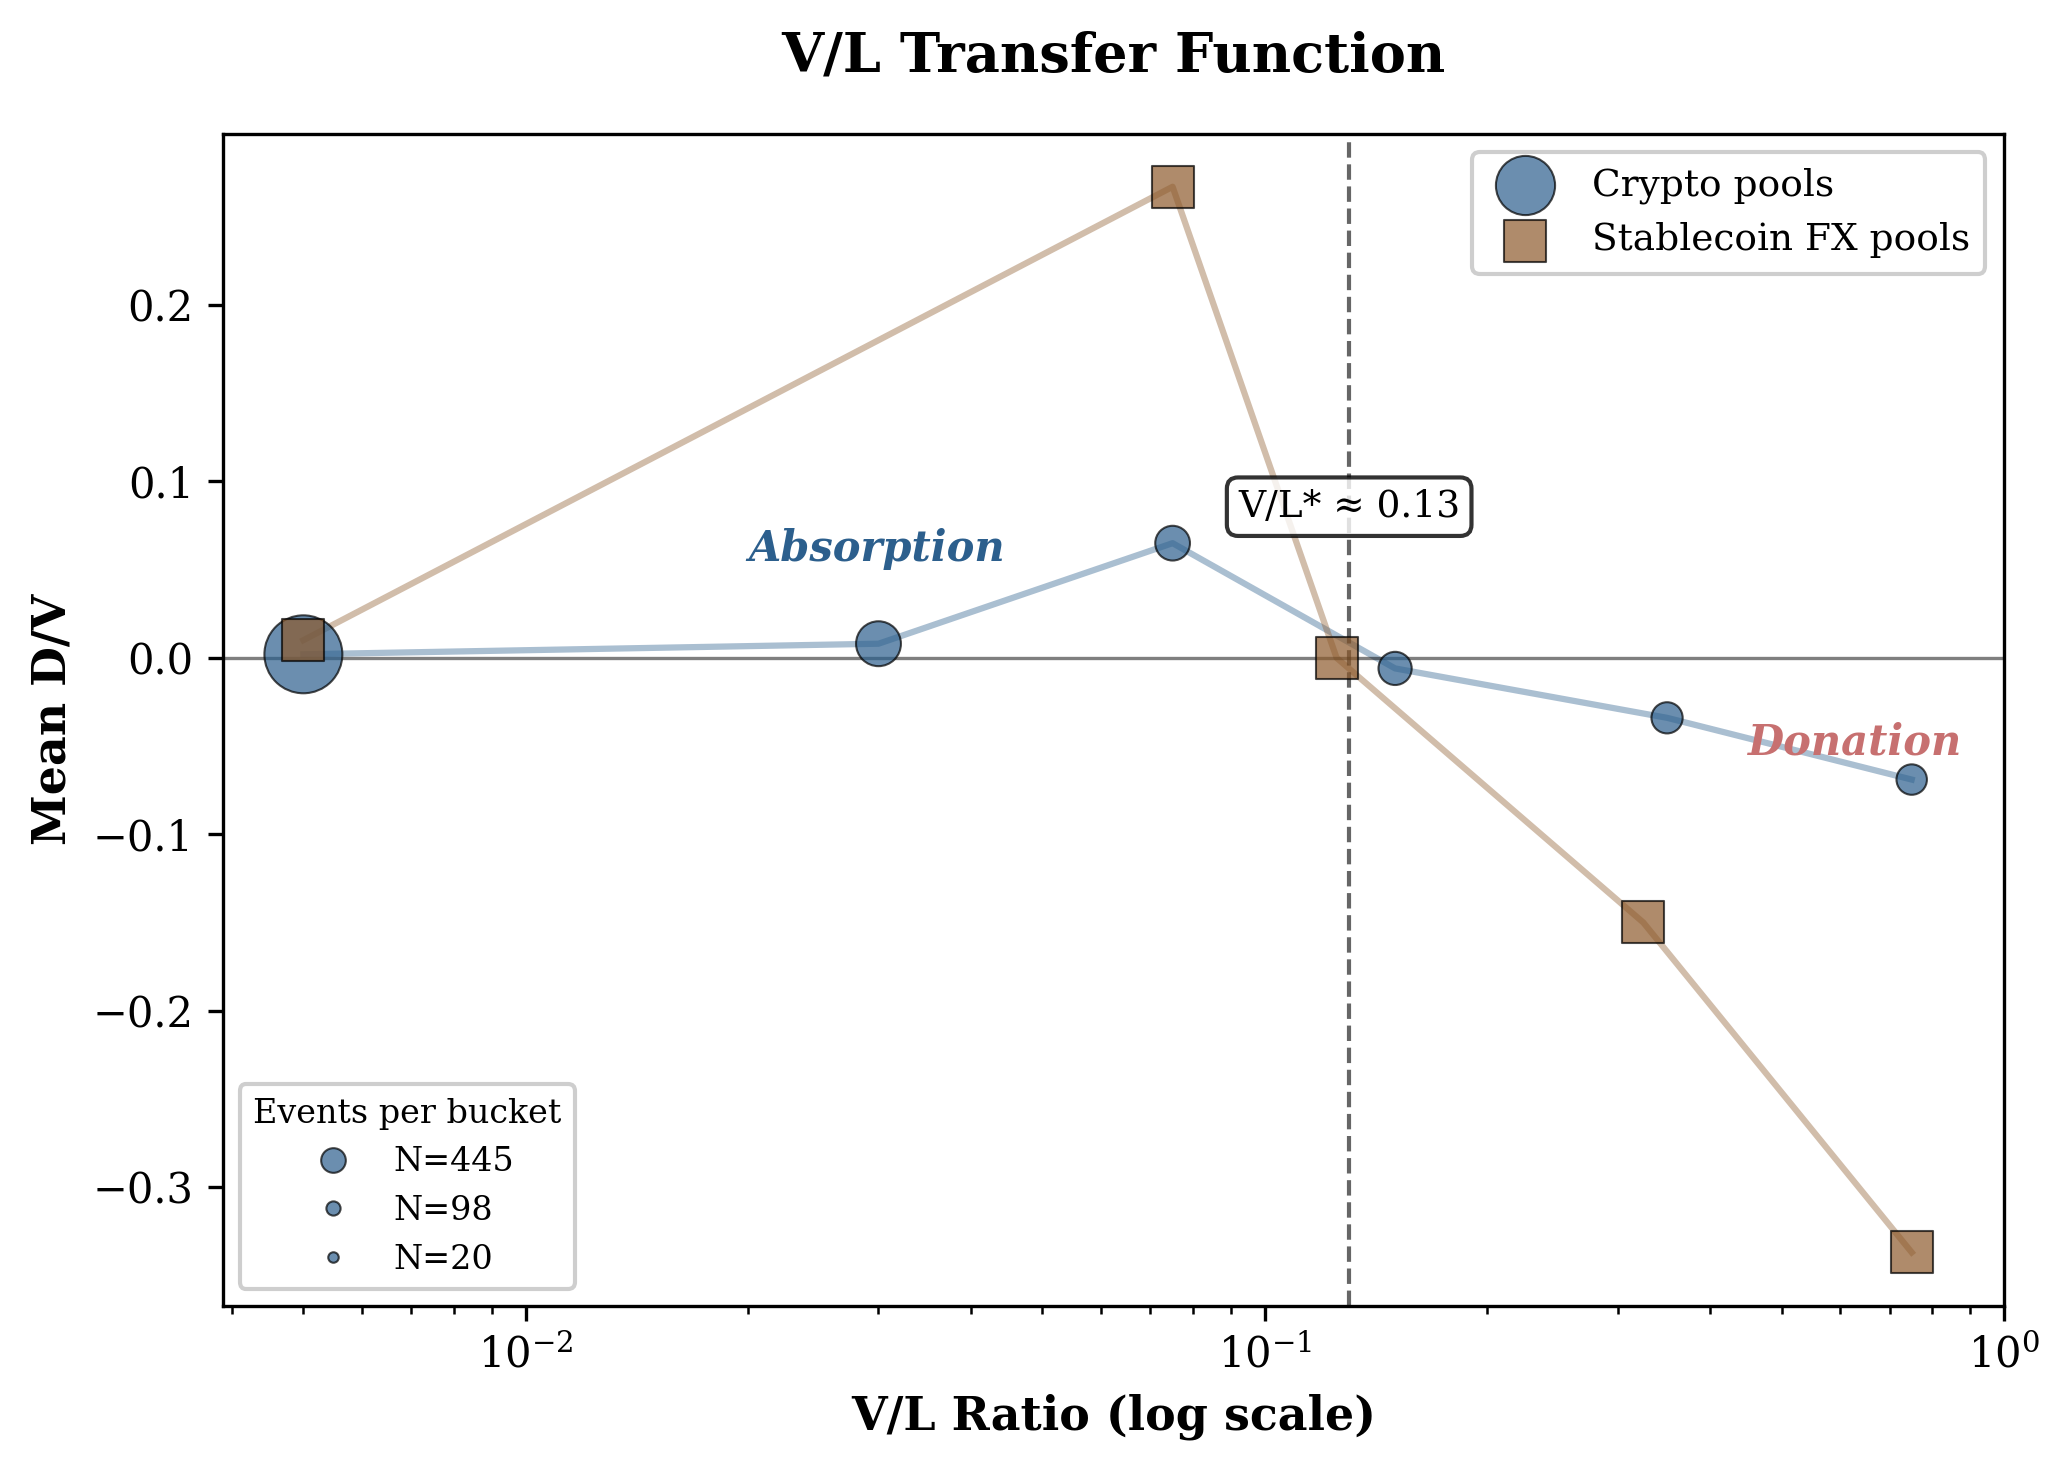
\includegraphics[width=0.8\linewidth,keepaspectratio]{figures/fig1-vl-transfer.png}
\caption{$V/L$ transfer function: absorption peaks at $V/L \approx 0.05$--$0.10$, crosses zero near $V/L^* \approx 0.13$, and donation intensifies above. Crypto pools (circles) and stablecoin FX pools (squares) shown; marker size proportional to $N$.}
\label{fig:vl-transfer}
\end{figure}

The peaked shape reflects the two-mechanism structure. At very low $V/L$, positions are too small for contract dust to materially affect them; at moderate $V/L$ ($0.05$--$0.10$), dust absorption is proportionally large; above the crossover $V/L^* \approx 0.13$, positions donate more than they absorb. The $73\%$ of events at $V/L < 0.01$ make linear regression misleading ($r \approx -0.1$), but the directional relationship is clear across the full range.

\textbf{$\sigma$ amplifies magnitude} ($\rho = +0.26$ for $\sigma_{1h}$ vs $|D/V|$, $N = 536$) but does not determine direction. High $\sigma$ + high $V/L$ compounds donation; high $\sigma$ + low $V/L$ compounds absorption.

\subsubsection*{Cross-group token decomposition}

Token-level decomposition of 395 transaction receipts across 10 pools and 5 depositor groups confirms the Connector Rule (\S\ref{sec:connector}):

\begin{table}[H]
\centering
\begin{tabular}{@{}llcrrr@{}}
\toprule
Pool & Group & Driver token & Driver $r$ & Other $r$ & $N$ \\
\midrule
CLAWD/USDC          & A & CLAWD       & \textbf{$-0.98$} & $-0.42$ & 62 \\
WETH/USDC           & A & WETH        & \textbf{$-0.98$} & $-0.31$ & 38 \\
WETH/AERO           & A & AERO        & \textbf{$-0.94$} & $-0.28$ & 31 \\
WETH/VVV            & B & WETH        & \textbf{$-0.89$} & $-0.15$ & 47 \\
WETH/AERO           & B & WETH        & \textbf{$-0.97$} & $-0.27$ & 73 \\
WETH/USDC           & B & USDC        & $-0.56$           & $-0.40$ & 25 \\
EURC/USDC           & C & USDC        & $-0.55$           & ---     & 9  \\
WETH/USDC           & D & USDC        & \textbf{$-0.68$} & $-0.56$ & 17 \\
KellyClaude/USDC    & E & KellyClaude & \textbf{$-0.68$} & $-0.60$ & 20 \\
\bottomrule
\end{tabular}
\end{table}

The WETH/USDC pool appears with three different depositor groups. In A (WETH is the connector), WETH drives at $r = -0.98$. In B (USDC is the connector), USDC drives at $r = -0.56$. The driver changes depending on what other pools share the depositor group.

\subsection{Single-pool equilibrium: the $V/L$ sweep}\label{sec:vl-sweep}

Three positions deployed in KellyClaude/USDC CL200 (${\sim}\$9{,}500$ TVL) at ratio $1{:}3{:}9$:

\begin{table}[H]
\centering
\begin{tabular}{@{}llrrl@{}}
\toprule
Position & Deployment & After 33 events & Dust PnL & Role \\
\midrule
Small  & \$199 ($V/L = 0.021$)   & ${\sim}\$900$ & \textbf{$+\$737$} & Absorber \\
Medium & \$597 ($V/L = 0.063$)   & ${\sim}\$656$ & $+\$84$           & Neutral (flipped) \\
Large  & \$1{,}799 ($V/L = 0.189$) & ${\sim}\$784$ & \textbf{$-\$933$} & Donor \\
\bottomrule
\end{tabular}
\end{table}

Deployment ratio $1{:}3{:}9 \to$ ratio at event 33: \textbf{$1.37{:}1{:}1.20$}. The original size ordering has reversed, and Small is now the largest position.

\begin{figure}[H]
\centering
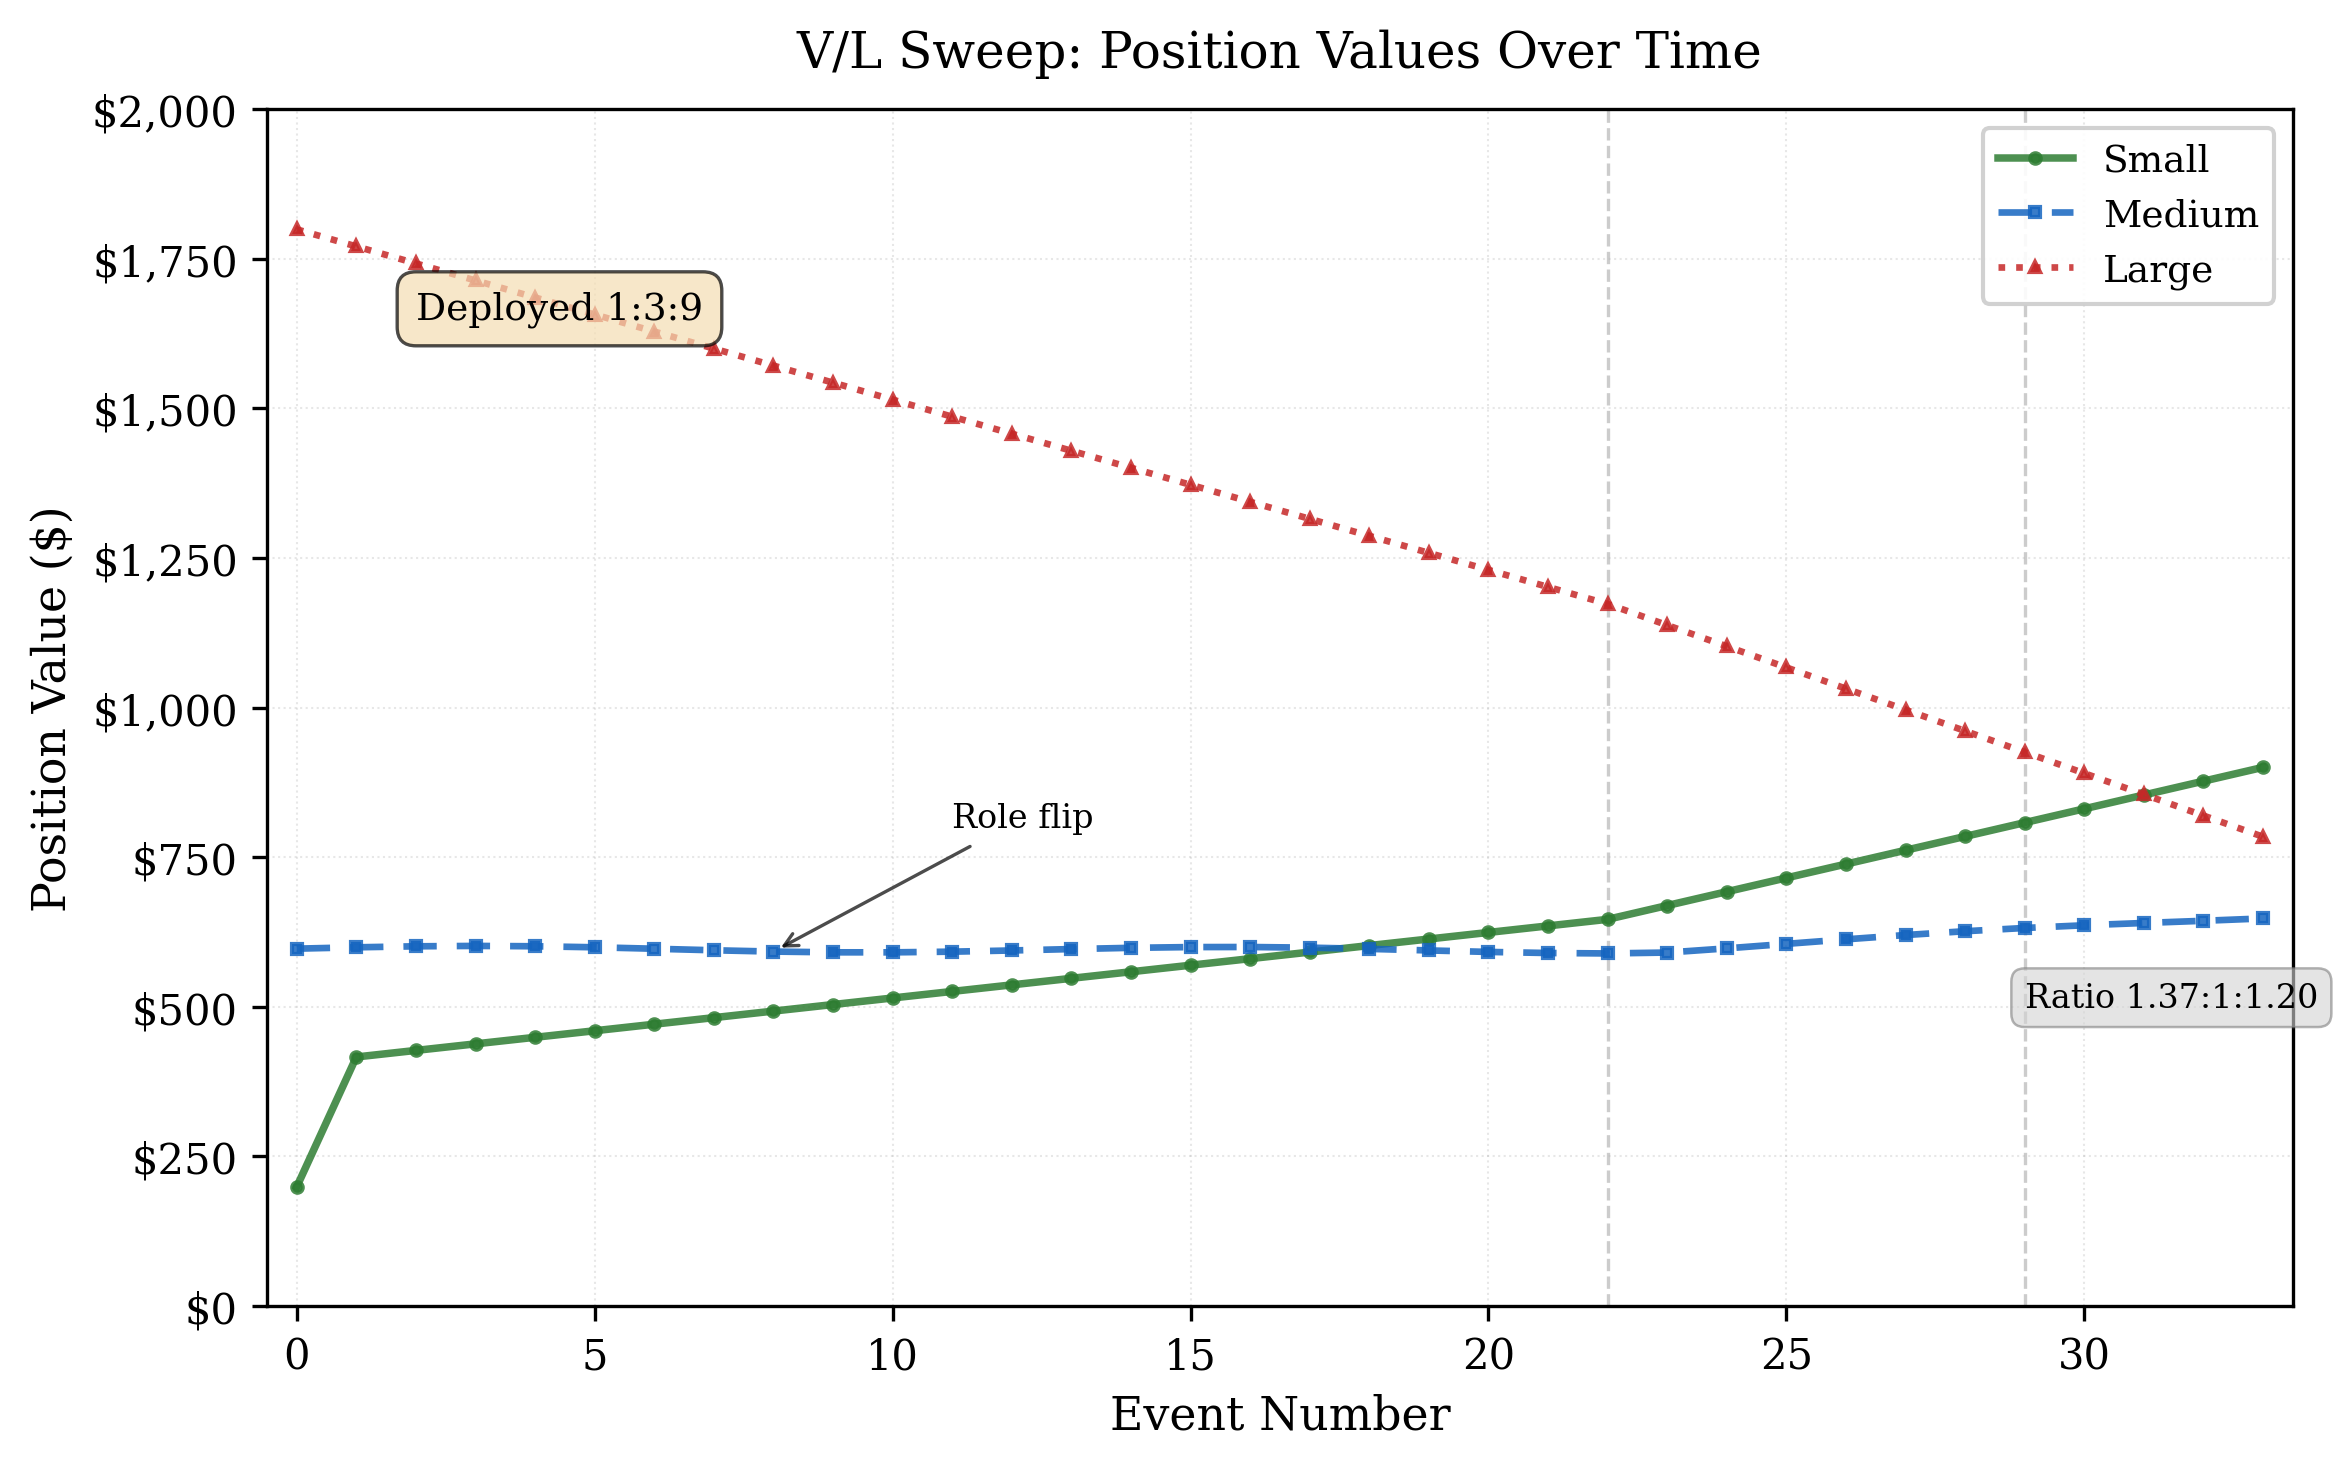
\includegraphics[width=0.8\linewidth,keepaspectratio]{figures/fig2-vl-sweep.png}
\caption{Single-pool convergence: three positions deployed at ratio $1{:}3{:}9$ converge towards near-equality over 33 diffusion events. Medium role-flips from donor to absorber at event ${\sim}8$. Original ordering reverses by event ${\sim}28$.}
\label{fig:vl-sweep}
\end{figure}

Medium role-flipped from initial donor to net absorber after 8 events.

\textbf{First-rebalance absorption.} The first automated rebalance absorbed all contract dust (\$217 from initial tightening) into the Small position --- a $114\%$ value increase in one event. The CL mint function uses all available tokens~\eqref{eq:mint}, creating winner-take-all dynamics on a per-event basis. Over many events, the probabilistic argument of Theorem~\ref{thm:convergence} prevails, and all positions converge.

\textbf{Transfer function.} Cross-validated with 33 fiat FX events ($N = 55$ total, $r = -0.528$):

\begin{table}[H]
\centering
\begin{tabular}{@{}llp{6.5cm}@{}}
\toprule
$V/L$ range & Mean $D/V$ & Behaviour \\
\midrule
$< 0.01$       & Weak positive    & Position too small to absorb meaningfully \\
$0.05$--$0.10$ & \textbf{$+0.267$} & Peak absorption (sweet spot) \\
$0.10$--$0.15$ & ${\sim}0$        & Crossover zone \\
$0.15$--$0.50$ & Negative          & Consistent donation \\
$0.50$--$1.0$  & \textbf{$-0.337$} & Massive donation (position dominates pool) \\
\bottomrule
\end{tabular}
\end{table}

The crossover $V/L^* \approx 0.13$--$0.15$ in liquidity ratio terms. CADC/USDC confirms this independently: pool TVL fluctuated around a fixed-size position, causing $V/L$ to traverse $0.003$ to $0.32$ and the position to role-flip multiple times at the crossover boundary.

\subsection{Multi-pool dynamics: hub-spoke topology}\label{sec:hub-spoke}

\begin{figure}[H]
\centering
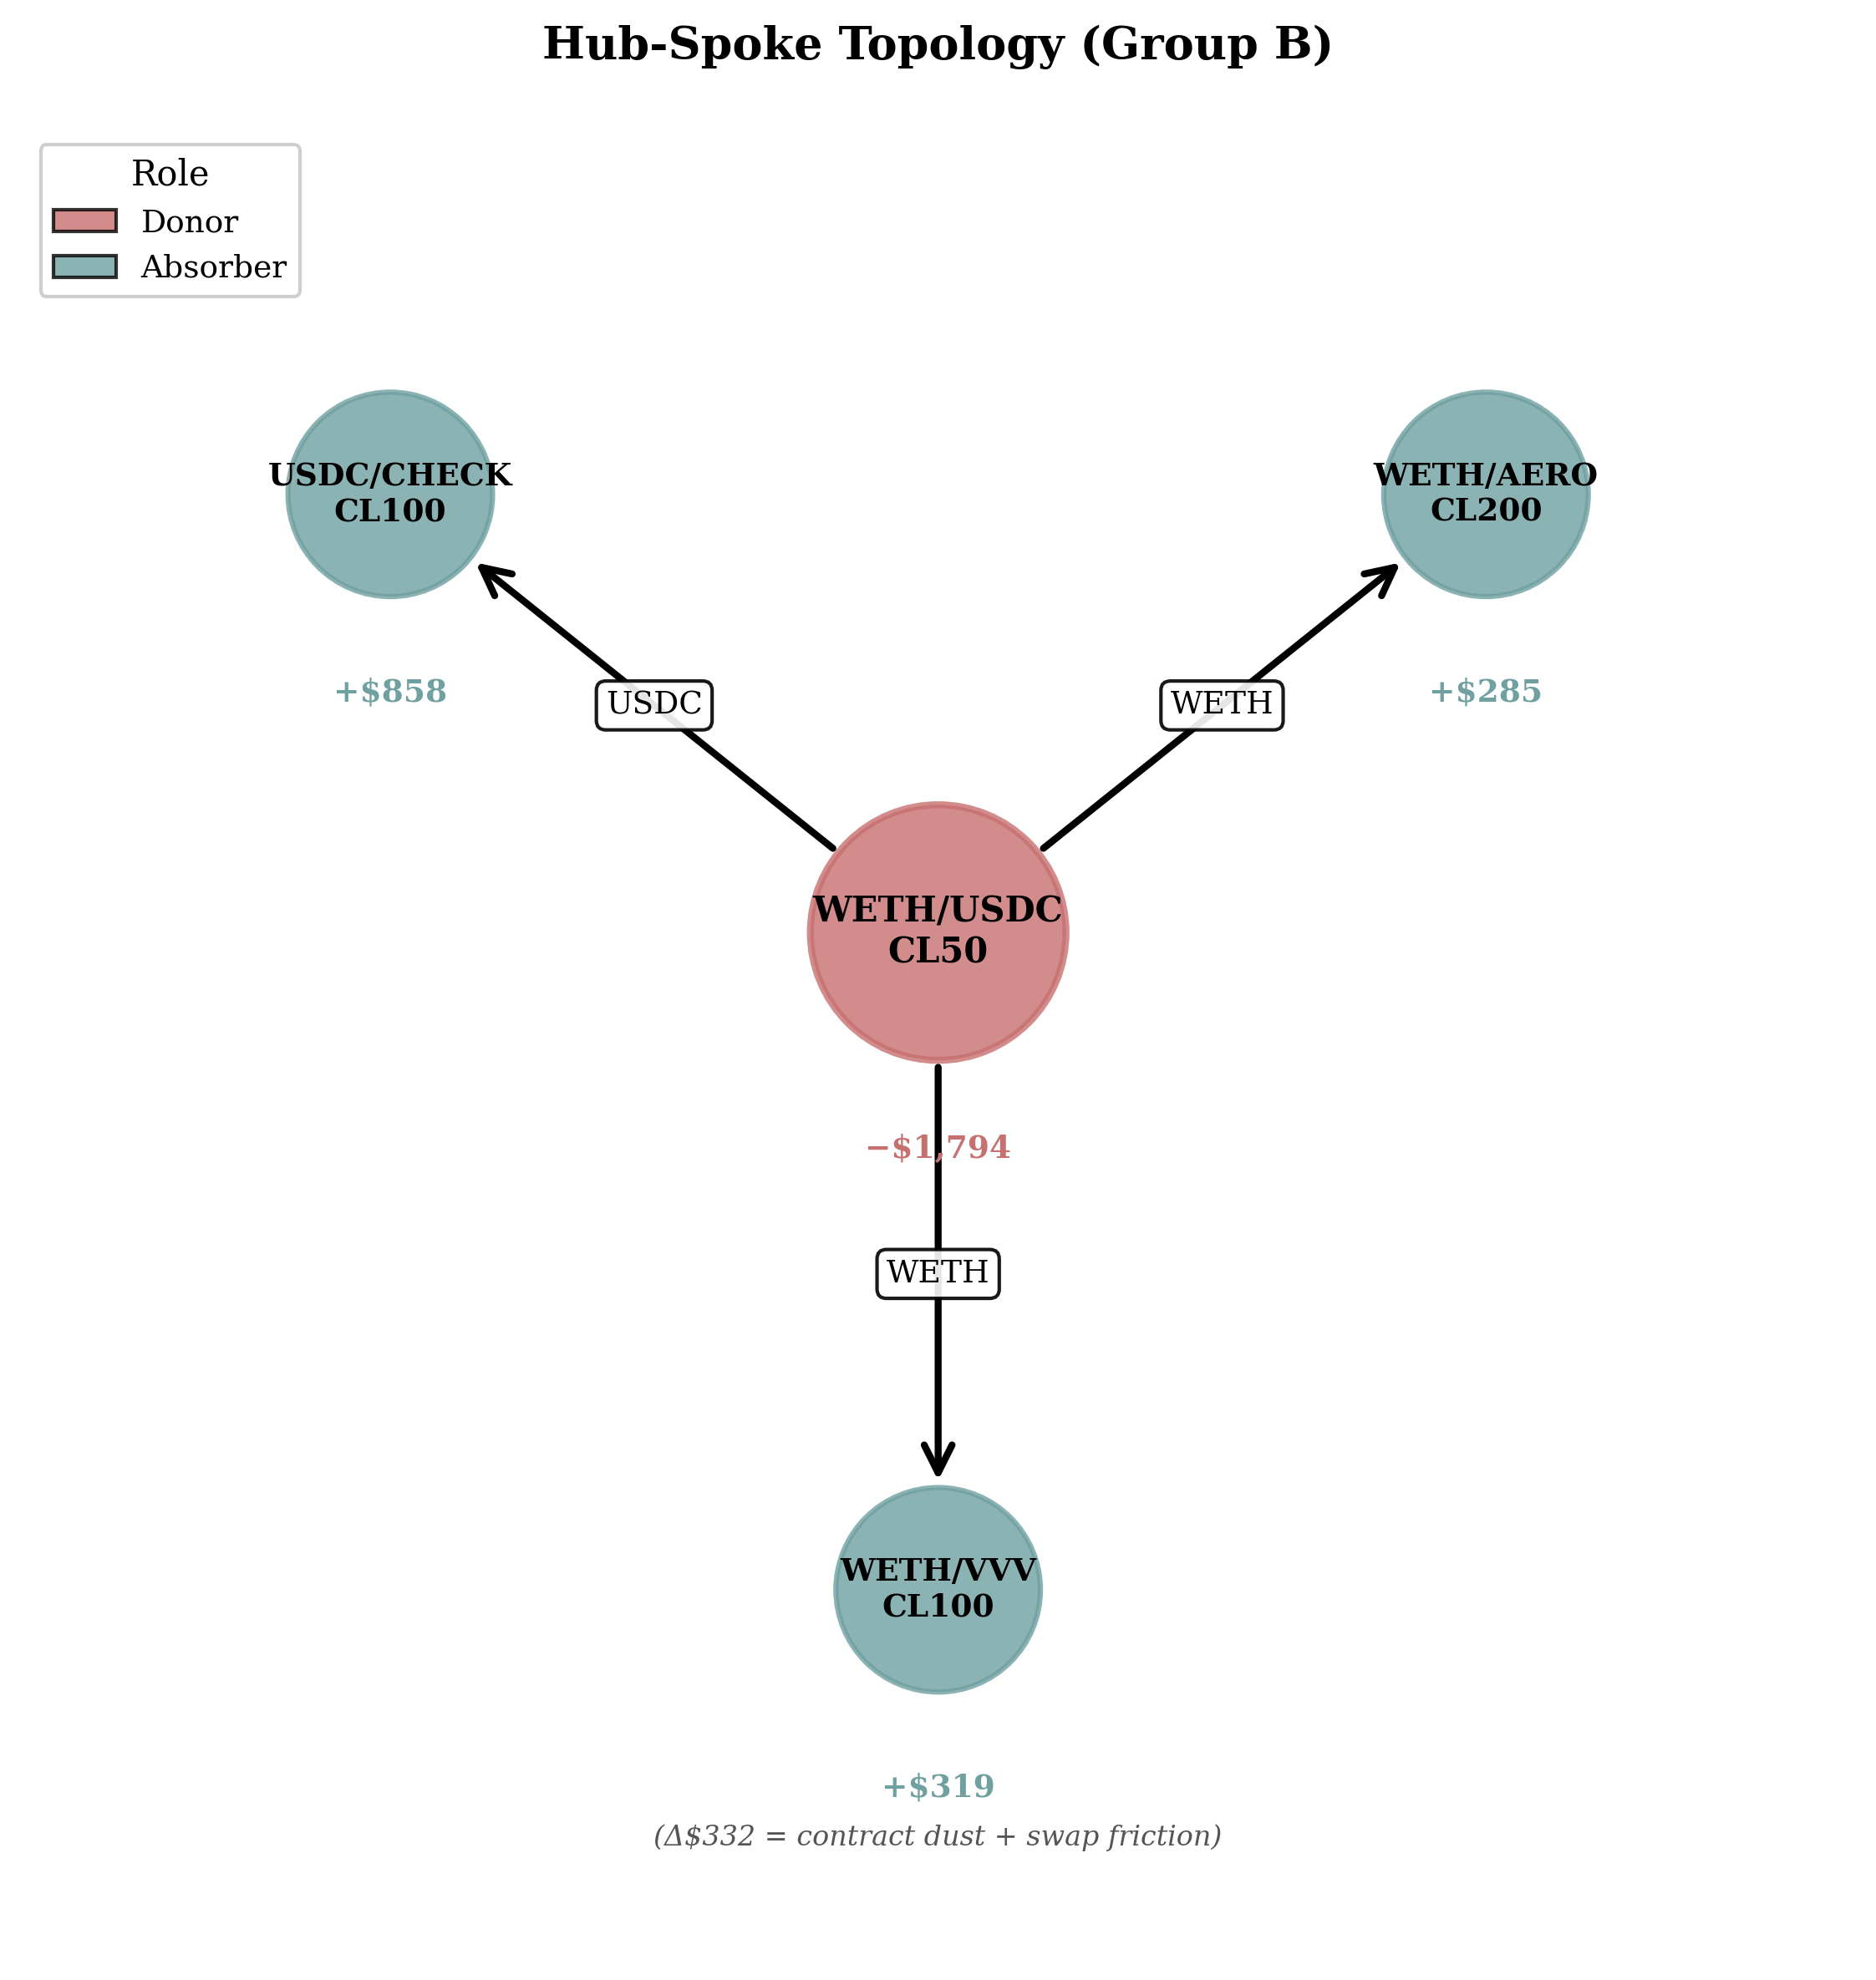
\includegraphics[width=0.6\linewidth,keepaspectratio]{figures/fig3-hub-spoke.png}
\caption{Hub-spoke topology (Group B): the WETH/USDC hub donates capital through shared WETH and USDC balances to three spoke positions. $\Delta\$332 = $ contract dust $+$ swap friction.}
\label{fig:hub-spoke}
\end{figure}

Phase 2's deliberate hub-spoke design with WETH/USDC CL50 as central hub:

\textbf{Group B (301 events):}

\begin{table}[H]
\centering
\begin{tabular}{@{}llrr@{}}
\toprule
Position & Role & Cumulative dust & Events \\
\midrule
WETH/USDC CL50 (hub) & Donor    & \textbf{$-\$1{,}794$} & 26 \\
USDC/CHECK CL100     & Absorber & $+\$858$              & 153 \\
WETH/AERO CL200      & Absorber & $+\$285$              & 73 \\
WETH/VVV CL100       & Absorber & $+\$319$              & 49 \\
\bottomrule
\end{tabular}
\end{table}

The hub donated \$1{,}794 and the three spokes collectively absorbed \$1{,}462. The difference (\$332) is contract dust plus cumulative swap friction.

\textbf{Temporal causation.} Every major hub donation has a matching spoke absorption within 2 hours. The hub leaves WETH residuals in the shared balance, and WETH-paired spokes pick them up on their next rebalance.

\textbf{Multi-pool stability.} Unlike single-pool positions (which equalise), multi-pool positions do not converge to equal value. The hub maintains a larger position because WETH/USDC CL50 has deeper TVL (lower $V/L$ at the same capital). Equation~\eqref{eq:multipool} predicts this: equal $V/L$ across pools means position sizes proportional to pool depth.

\needspace{14\baselineskip}
\subsection{Regime analysis}\label{sec:regime}

The 41.9-hour Phase 1 observation spans five distinct market phases:

\begin{table}[H]
\centering
\begin{tabular}{@{}llrrl@{}}
\toprule
Phase & Period (UTC) & Events & Net \$ & Character \\
\midrule
P1: Stress      & 03 Mar 17:49 -- 04 Mar 06:00 & 217 & $-\$196$ & ETH \$2{,}215 $\to$ \$1{,}984 \\
P2: Recovery    & 04 Mar 06:00 -- 12:00         & 137 & $+\$960$ & Volatility subsides \\
P3: Rally       & 04 Mar 12:00 -- 20:45         & 170 & $-\$240$ & BTC $\to$ \$71.4K \\
P4: Post-Rally  & 04 Mar 20:45 -- 05 Mar 04:34  & 147 & $-\$323$ & Consolidation \\
P5: Calm        & 05 Mar 04:34 -- 11:47         & 67  & $+\$86$  & Diverse portfolios stabilise \\
\bottomrule
\end{tabular}
\end{table}

\textbf{Regime-dependent roles.} During stress (P1), volatile positions shed capital as geometric mismatches widen. During the rally (P3), the same positions absorb. No position is permanently a donor or absorber.

\subsection{Stablecoin FX isolation}\label{sec:fx-isolation}

Five stablecoin FX pairs deployed on a Sunday (markets closed, $\sigma \approx 0$) provide a natural control experiment isolating $V/L$ from volatility:

\begin{table}[H]
\centering
\begin{tabular}{@{}lrrrr@{}}
\toprule
Position & $V/L$ & $\sigma_{24h}$ & Cumulative dust & Swaps \\
\midrule
ZARP & 0.958 & 98.8 & \textbf{$-\$601$} & 0 \\
VCHF & 0.034 & 1.4  & $+\$72$            & 0 \\
CADC & 0.003 & 5.0  & $+\$131$           & 0 \\
KRWQ & 0.025 & 1.5  & $+\$432$           & 0 \\
EURC & 0.001 & 0.1  & $+\$216$           & 0 \\
\bottomrule
\end{tabular}
\end{table}

\textbf{Zero swaps} across all fiat rebalances (\texttt{amountIn = 0} in every \texttt{rebalanceCL} call). All dust flow is pure geometric residual $\Delta R$ with no swap friction component.

ZARP ($V/L \approx 0.96$, meaning the position accounts for nearly all the pool's liquidity) donated a mean $27\%$ of its value per donation event. All five FX pairs were deployed with equal capital. ZARP shrank steadily ($V/L$: $0.958 \to 0.974 \to 0.992$) whilst KRWQ and CADC grew. Capital was conserved at portfolio level.

FX markets were closed and no swaps occurred in any fiat rebalance. Every observed capital flow is therefore attributable to CL geometry alone, confirming $V/L$ as the sole predictor when $\sigma$ is eliminated.

\subsection{Formula verification: the two-mechanism split}\label{sec:two-mechanism-split}

\begin{figure}[H]
\centering
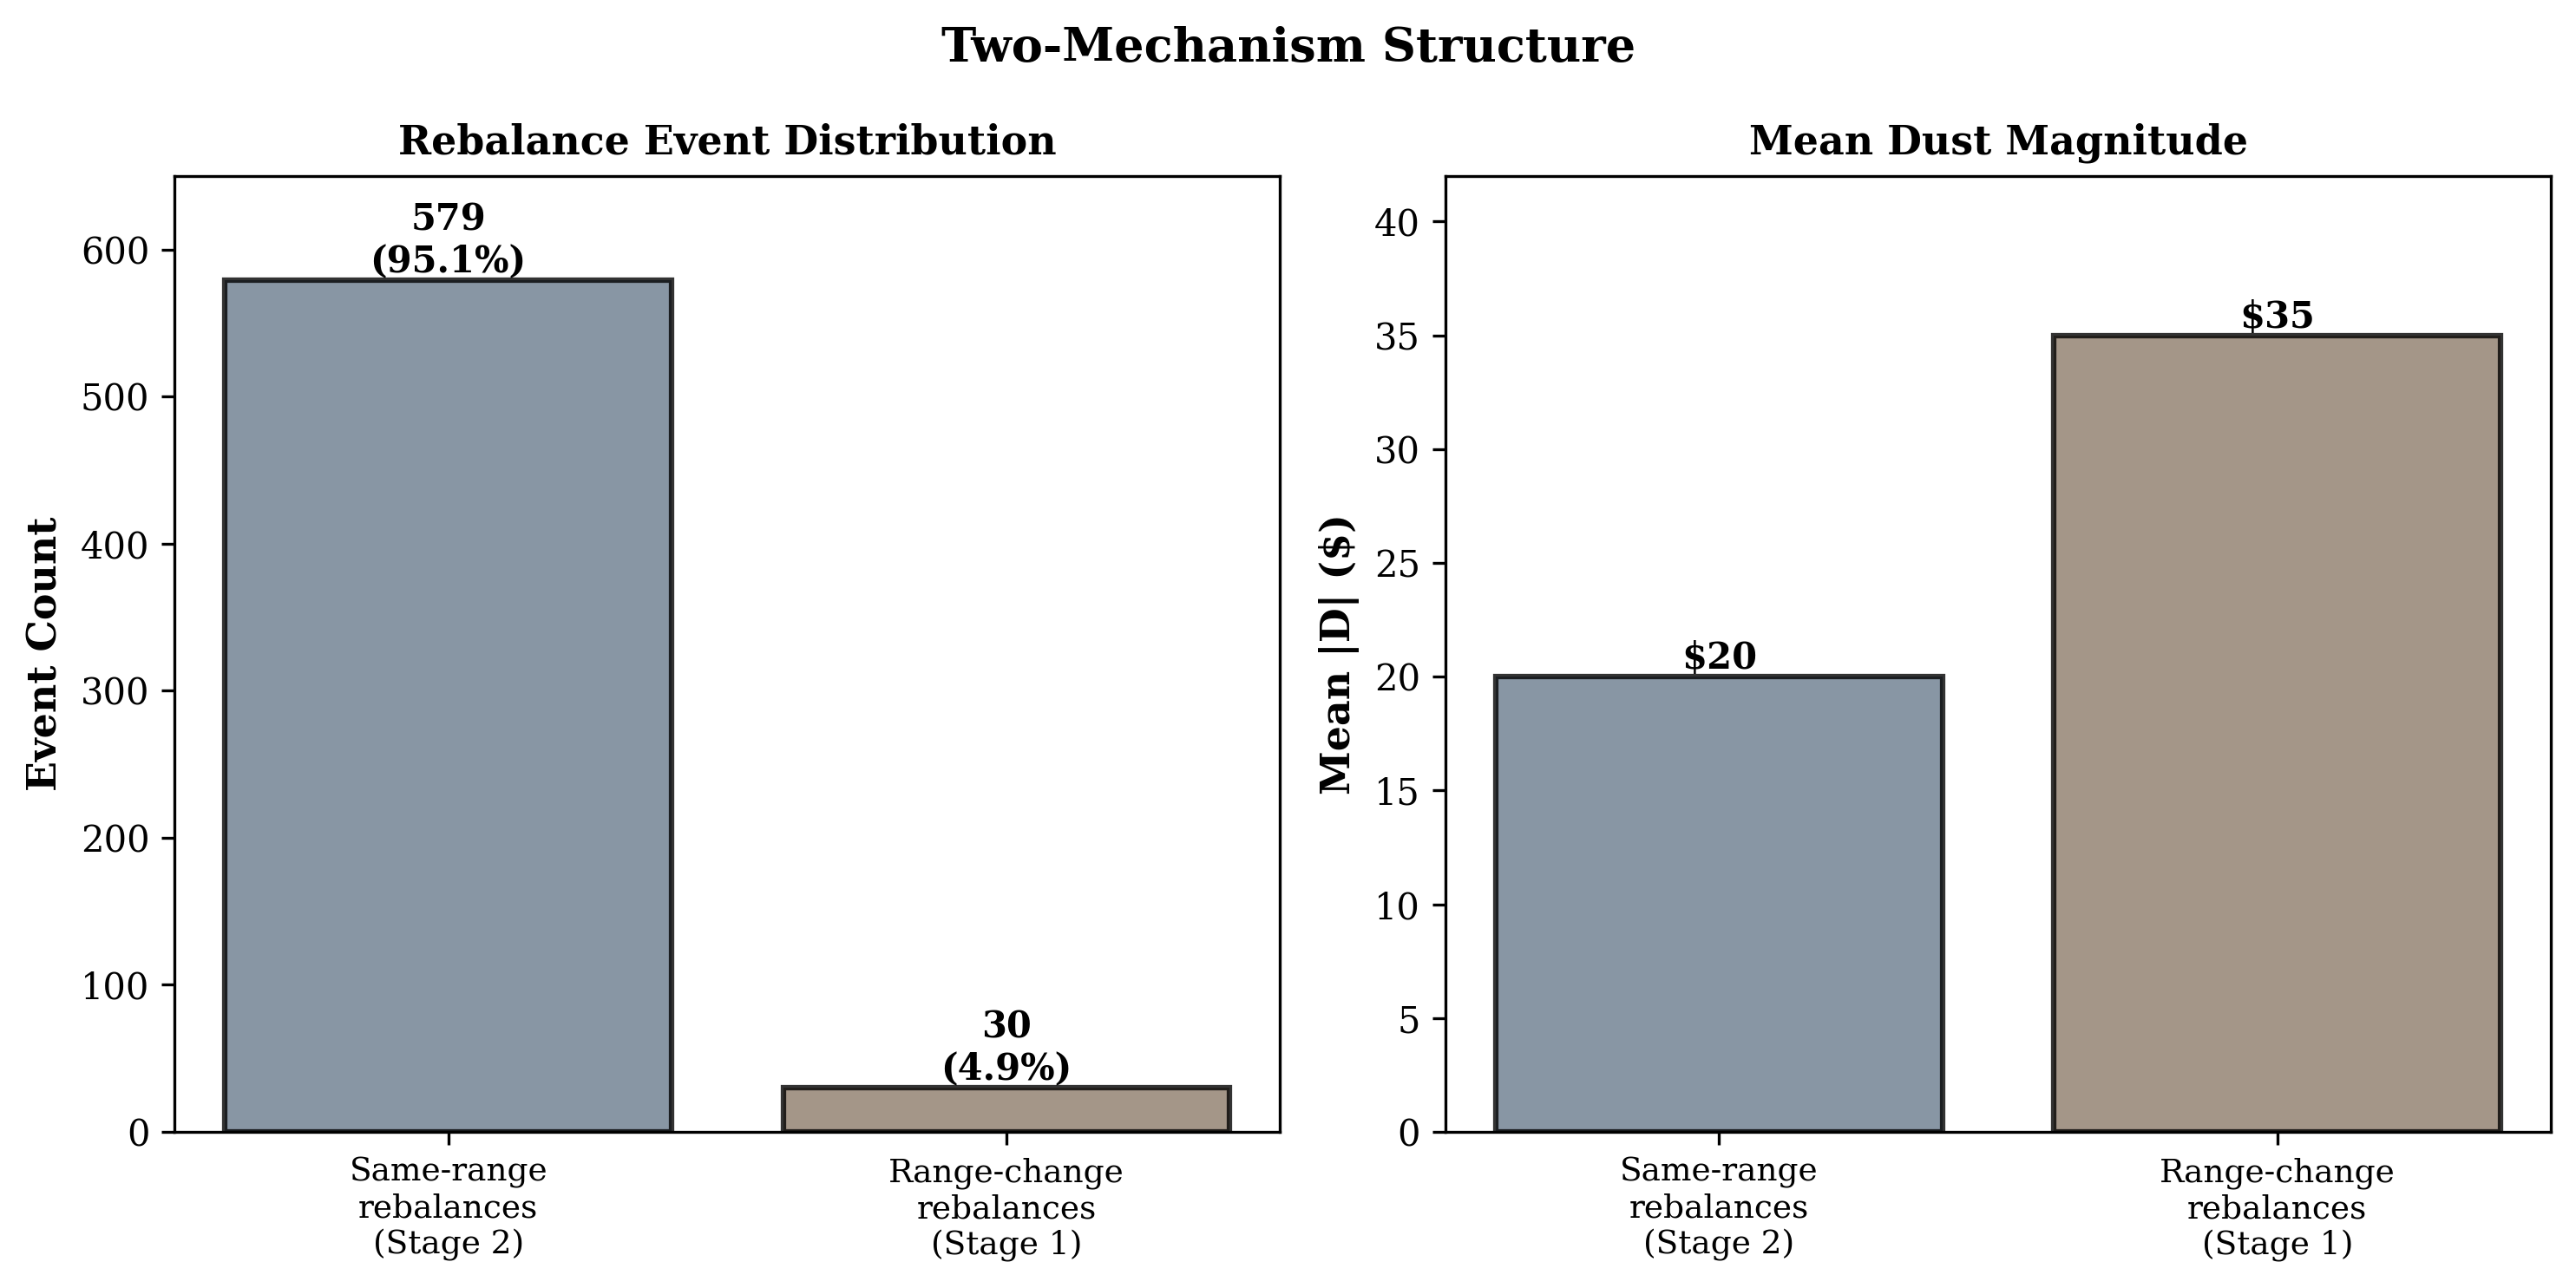
\includegraphics[width=0.85\linewidth,keepaspectratio]{figures/fig4-two-mechanism.png}
\caption{Two-mechanism structure: $95\%$ of events are same-range rebalances (Stage~2, dust redistribution) with mean $|D| = \$20$; $5\%$ are range changes (Stage~1, geometric creation) with mean $|D| = \$35$.}
\label{fig:two-mechanism}
\end{figure}

Verification of the closed-form $D/V$ against 642 Phase 2 events:

\begin{table}[H]
\centering
\begin{tabular}{@{}lrlll@{}}
\toprule
Category     & Events     & Range changes? & $\Delta R = 0$? & Mean $|D|$ \\
\midrule
Same-range   & 611 (95\%) & No             & Yes (all 611)    & \$20 \\
Range-change & 31 (5\%)   & Yes            & No (all 31)      & \$35 \\
\bottomrule
\end{tabular}
\end{table}

\textbf{Same-range confirmation.} All 611 same-range events have $\Delta R = 0$ as predicted by Theorem~\ref{thm:residual}. Their non-zero dust flows ($\overline{|D|} = \$20$) are entirely Stage~2 (dust pool redistribution).

\textbf{Range-change confirmation.} All 31 range-change events have $\Delta R \neq 0$. Of the 28 events where the current tick was within the old range (permitting unambiguous case assignment), the formula predicts the direction correctly in 19 cases ($70\%$). Magnitude comparison: predicted $|\overline{D/V}| = 44\%$, actual $|\overline{D/V}| = 2.7\%$. The internal swap absorbs ${\sim}94\%$ of the gross geometric mismatch, leaving ${\sim}6\%$ as net dust. The formula describes the gross geometric residual; the swap partially offsets it but does not eliminate it.

\subsection{Position extinction: the ZARP case study}\label{sec:zarp}

The USDC/ZARP CL10 position provides a complete empirical lifecycle of Theorem~\ref{thm:extinction}, from deployment to extinction, with $S = 0$ on every event.

ZARP (South African Rand stablecoin) had no DEX swap routing. The Odos aggregator returned no path. Every rebalance was a pure withdraw $\to$ mint with no token ratio correction, so $D = \Delta R$ exactly. This isolates the geometric residual with no swap confounders.

\begin{table}[H]
\centering\small
\begin{tabular}{@{}rlrrrrrr@{}}
\toprule
Event & Time (UTC) & Pre (\$) & Post (\$) & Dust $D$ & $V/L$ & $\alpha$ & Pool $\mathcal{L}$ \\
\midrule
1  & 07 Mar 17:05 & 942 & 791  & $-151$              & 0.958          & 0.16            & 135M \\
2  & 07 Mar 19:30 & 791 & 532  & $-259$              & 0.974          & 0.33            & 223M \\
3  & 08 Mar 05:02 & 532 & 338  & $-194$              & 0.992          & 0.36            & 693M \\
4  & 08 Mar 13:27 & 338 & 170  & $-168$              & 0.960          & 0.50            & 144M \\
5  & 08 Mar 22:31 & 170 & 342  & \textbf{$+172$}     & 0.790          & ---             & 352M \\
6  & 09 Mar 00:24 & 342 & 171  & $-171$              & 0.598          & 0.50            & 232M \\
7  & 09 Mar 04:37 & 170 & 51   & $-119$              & 0.448          & 0.70            & 93M \\
8  & 09 Mar 04:46 & 51  & 281  & \textbf{$+230$}     & 0.976          & ---             & 235M \\
9  & 09 Mar 10:18 & 280 & 235  & $-45$               & 0.971          & 0.16            & 197M \\
10 & 09 Mar 11:08 & 235 & 188  & $-47$               & 0.966          & 0.20            & 158M \\
11 & 09 Mar 13:47 & 187 & 77   & $-110$              & 0.917          & 0.59            & 68M \\
12 & 09 Mar 16:40 & 77  & 248  & \textbf{$+171$}     & 0.152          & ---             & 1{,}341M \\
13 & 09 Mar 21:28 & 249 & 264  & $+15$               & 0.159          & ---             & 1{,}353M \\
14 & 10 Mar 09:52 & 264 & \textbf{1.59} & $-262$     & \textbf{0.001} & \textbf{0.99}   & 1{,}137M \\
\bottomrule
\end{tabular}
\end{table}

Swaps executed: \textbf{0 of 14}. Total donated: \$1{,}526. Total absorbed: \$588 (4 events). Net: $-\$938$ ($99.8\%$ of capital).

\textbf{Three phases.} Events 1--4: the position dominated the pool ($V/L > 0.95$) and donated on every rebalance. Events 5--8: $\mathcal{L}$ fluctuated by $4\times$, producing alternating donation and absorption. Events 9--14: $\mathcal{L}$ increased $20\times$ between events 11 and 12, reducing $V/\mathcal{L}$ to $0.001$. The final rebalance produced $\alpha = 0.99$.

\textbf{Extinction bound.} Using Theorem~\ref{thm:extinction}'s formula with $\alpha_{\min} = 0.16$ (Event 1, smallest donation):
\[
K^* = \left\lceil \frac{\ln(942/1.59)}{\ln(1/0.84)} \right\rceil = \lceil 36.7 \rceil = 37 \text{ rebalances}.
\]
Using $\alpha_{\text{avg}} = 0.45$ across the 10 donation events:
\[
K^* = \left\lceil \frac{\ln(942/1.59)}{\ln(1/0.55)} \right\rceil = \lceil 10.7 \rceil = 11 \text{ rebalances}.
\]

Theorem predicts 11 rebalances at average leak rate; 10 donation events were observed (the remaining 4 were absorptions from exogenous liquidity changes). The bound matches the observed trajectory closely.

\textbf{Corollary validation.} The three largest absorption events (5, 8, 12) each coincided with a substantial increase in pool liquidity $\mathcal{L}$. After each absorption, the position returned to donation on the subsequent rebalance, consistent with the irreversibility corollary.

\begin{center}\rule{0.5\linewidth}{0.5pt}\end{center}

\section{Independent verification: Foundry proof}\label{sec:foundry}

The closed-form derivation is verified with a Foundry test suite covering both Theorem~\ref{thm:residual} (geometric residual existence and scaling, \S\ref{sec:foundry-mock-residual}) and Theorem~\ref{thm:extinction} (zero-swap extinction, \S\ref{sec:foundry-mock-extinction}). Two complementary verification surfaces are used:

\begin{itemize}[leftmargin=*]
    \item \textbf{Mock-pool tests} (\texttt{MockCLPool}), which implement the Uniswap V3 amount equations against a self-contained pool with a linearised tick-to-sqrt-price approximation. These exercise the residual geometry in isolation, with no fees, no slippage, and no dependence on a live RPC endpoint, but are not Uniswap-accurate in the last significant figure.
    \item \textbf{Fork tests} against unmodified Aerodrome Slipstream contracts on Base mainnet via Foundry's \texttt{vm.createSelectFork}, exercising the same scenarios on real on-chain V3 geometry. These give the canonical demonstration that the residual is a property of unmodified V3 contracts, with the trade-off that the numerical residuals are non-deterministic between runs as the live pool state shifts.
\end{itemize}

The mock-pool and fork-pool surfaces verify the same theorem at different displacement magnitudes; their qualitative agreement (residual exists, control case is dust-only, residual scales with size) is the central reproducibility claim. \S\ref{sec:foundry-mock-residual}--\S\ref{sec:foundry-mock-extinction} report the mock-pool numbers because they are deterministic and small enough to quote directly; \S\ref{sec:foundry-fork} reports the fork-pool verification.

\subsection{Test 1: Range change creates residual}\label{sec:foundry-mock-residual}

\begin{table}[H]
\centering
\begin{tabular}{@{}ll@{}}
\toprule
Step & Value \\
\midrule
Initial position & 1 WETH $+$ 2{,}500 USDC, $\pm 500$ ticks around tick 73{,}135 \\
Price movement   & $+200$ ticks \\
New range        & $\pm 1{,}000$ ticks (wider) \\
Withdrawn        & 0.076 WETH $+$ 3{,}434 USDC \\
Minted           & 6{,}681M liquidity (from 23{,}525M) \\
\textbf{Residual} & \textbf{2{,}061 USDC} returned to depositor balance \\
\bottomrule
\end{tabular}
\end{table}

Assertion: \texttt{assertTrue(residual0 > 0 || residual1 > 0)} --- \textbf{PASSED}.

\subsection{Test 2: Same range = zero residual (control)}\label{sec:foundry-mock-control}

Same setup, same price movement, but re-mint into the \textbf{identical range}. Residual: \textbf{29 wei} ($< 10^{-6}$ USD). Pure integer rounding from the Solidity floor division in the mint constraint.

Assertion: \texttt{assertLt(residual1, 1e3)} --- \textbf{PASSED}. This confirms the converse of Theorem~\ref{thm:residual}: $R_{\text{old}} = R_{\text{new}} \Rightarrow \Delta R = 0$.

\subsection{Test 3: Linear scaling with position size}\label{sec:foundry-mock-scaling}

\begin{table}[H]
\centering
\begin{tabular}{@{}lrl@{}}
\toprule
Position size & Residual (raw) & Ratio \\
\midrule
0.5 WETH & 1{,}030 & $1.0\times$ \\
2.0 WETH & 4{,}122 & \textbf{$4.00\times$} \\
\bottomrule
\end{tabular}
\end{table}

$4\times$ position $\to$ $4\times$ residual. The $D/V$ ratio depends on tick displacement and range width, so it scales linearly with position size. Consistent with equations~\eqref{eq:caseA}--\eqref{eq:caseB} where $V_{\text{new}}/V_{\text{old}}$ is independent of $L$.

Assertion: \texttt{assertGt(largeResidual, smallResidual)} --- \textbf{PASSED}.

\subsection{What tests 1--3 establish}\label{sec:foundry-mock-summary}

\begin{enumerate}[leftmargin=*]
    \item The residual appears against an isolated implementation of the Uniswap V3 amount equations with no additional infrastructure, confirming it originates in the CL curve geometry rather than in any contract-level logic.
    \item Same-range rebalances produce zero residual ($611/611$ events in the empirical dataset, see \S\ref{sec:two-mechanism-split}), confirming the converse of Theorem~\ref{thm:residual}.
    \item A $4\times$ position produces a $4\times$ residual (ratio $4.00$), so the $D/V$ formulation is well-defined and independent of $L$ in the range where $\phi$ is approximately linear.
\end{enumerate}

The mock pool used by tests 1--3 implements a linearised \texttt{getSqrtRatioAtTick} approximation around tick 73{,}135. This is sufficient to demonstrate the existence and scaling of the residual at the order of magnitude reported above, but introduces small rounding artefacts (the $0.5$~WETH residual in Test~3 rounds down from a true value of $\sim 1{,}030.5$). For Uniswap-accurate quantitative verification of the same theorem, see the fork-pool results in \S\ref{sec:foundry-fork}.

\subsection{Test 4: Single-sided exit with no swap (Theorem~\ref{thm:extinction}, part i)}\label{sec:foundry-mock-extinction}

\begin{table}[H]
\centering
\begin{tabular}{@{}ll@{}}
\toprule
Step & Value \\
\midrule
Initial position & 1 WETH $+$ 2{,}500 USDC, range $[72800, 73000]$ \\
Price movement   & $+200$ ticks (above upper bound) \\
Withdrawal       & 0 WETH, 2{,}499{,}999{,}999 USDC ($100\%$ token1) \\
New range        & $[73000, 73400]$ (requires both tokens) \\
New liquidity    & \textbf{0} (token0 $= 0 \Rightarrow \min()$ constraint binds at zero) \\
\textbf{Residual} & \textbf{$100\%$ of position value} \\
\bottomrule
\end{tabular}
\end{table}

Assertion: \texttt{assertTrue(finalValue < initialValue)} --- \textbf{PASSED}. $\alpha = 1.0$: a fully single-sided withdrawal with no swap mints zero liquidity. The entire position becomes dust.

\subsection{Test 5: Residual scales with displacement (Theorem~\ref{thm:extinction}, part ii)}\label{sec:foundry-displacement}

Position deployed with $1{,}000$-tick range. Price displaced past the upper boundary by varying amounts:

\begin{table}[H]
\centering
\begin{tabular}{@{}lr@{}}
\toprule
Displacement & $\alpha$ \\
\midrule
100 ticks & $0\%$ \\
300 ticks & $37\%$ \\
600 ticks & $100\%$ \\
\bottomrule
\end{tabular}
\end{table}

Assertion: \texttt{assertTrue(alpha\_300 > alpha\_100 \&\& alpha\_600 > alpha\_300)} --- \textbf{PASSED}. Monotonic increase confirmed. The $\alpha = 0\%$ at 100 ticks reflects the mock pool's linear sqrt-price approximation; on real V3 tick math (and on the live fork test in \S\ref{sec:foundry-fork}), this would be small but strictly positive.

\subsection{Test 6: Geometric decay over repeated rebalances (Theorem~\ref{thm:extinction}, part iii)}\label{sec:foundry-decay}

Five sequential rebalance cycles with 150-tick price drift and no swap:

\begin{table}[H]
\centering
\begin{tabular}{@{}rrr@{}}
\toprule
Cycle & Value (USD) & Decay factor \\
\midrule
0 & 4{,}999 & --- \\
1 & 3{,}823 & 0.76 \\
2 & 1{,}565 & 0.40 \\
3 & 1{,}197 & 0.76 \\
4 & 490     & 0.40 \\
5 & 374     & 0.76 \\
\bottomrule
\end{tabular}
\end{table}

Assertion: \texttt{assertTrue(V[k+1] < V[k])} for all $k$ --- \textbf{PASSED}. Total decay: $92\%$ in 5 cycles. The alternating factor ($0.76 / 0.40$) reflects the token-ratio flip at each step. The two-step product $0.76 \times 0.40 = 0.30$ is the effective decay constant.

\subsection{Test 7: Deep out-of-range terminal event (Theorem~\ref{thm:extinction}, part ii extreme)}\label{sec:foundry-terminal}

\begin{table}[H]
\centering
\begin{tabular}{@{}ll@{}}
\toprule
Step & Value \\
\midrule
Initial position & $\pm 200$ ticks around tick 73{,}135 \\
Price movement   & $+2{,}000$ ticks past upper bound \\
New liquidity    & \textbf{0} \\
\textbf{$\alpha$} & \textbf{$100\%$} \\
\bottomrule
\end{tabular}
\end{table}

Assertion: \texttt{assertTrue(alpha > 95)} --- \textbf{PASSED}. At 2{,}000-tick displacement, the position is entirely single-sided. This mirrors the ZARP terminal event (Event 14, \S\ref{sec:zarp}: $\alpha = 0.99$).

\subsection{Live fork verification}\label{sec:foundry-fork}

The same scenarios are also run as fork tests against the live Aerodrome Slipstream WETH/USDC pool on Base mainnet, calling the unmodified \texttt{NonfungiblePositionManager} and pool contracts directly via \texttt{vm.createSelectFork}. Five tests reproduce the range-change residual, same-range control, wider-range case, $4\times$ scaling and the architectural precondition (\S\ref{sec:precondition}) against real on-chain V3 geometry.

Fork residuals are smaller than mock-pool residuals (${\sim}\$128$ vs ${\sim}\$2{,}061$) because the fork test swaps a fixed \$1{,}000 USDC to move the price, shifting the tick by only ${\sim}1$--$3$ ticks rather than the mock's hardcoded $+200$. The precondition test (\texttt{test\_stockNfpmDoesNotAbsorbDust}) creates two positions in the same range, leaves a residual via the first, then confirms the second's liquidity does not grow on a same-range rebalance. A stock NFPM has no shared dust balance, so no cross-position absorption occurs.

The fork tests do not pin a block number; numerical residuals shift between runs, but the qualitative claims hold deterministically.

\subsection{What the full suite establishes}\label{sec:foundry-summary}

Tests 1--3 prove Theorem~\ref{thm:residual} (geometric residual existence and scaling). Tests 4--7 prove Theorem~\ref{thm:extinction} (zero-swap extinction: single-step loss, monotonic displacement scaling, geometric decay, terminal events). The five fork tests in \S\ref{sec:foundry-fork} reproduce Tests 1, 2, 3 and the architectural precondition against unmodified live Slipstream contracts. The full suite runs in well under a second:

\begin{verbatim}
forge test -vv
Suite result: ok. 7 passed; 0 failed; 0 skipped  (mock-pool tests)
Suite result: ok. 5 passed; 0 failed; 0 skipped  (fork tests, requires Base RPC)
\end{verbatim}

The mock-pool environment has no swaps, zero fees, a single position, and no adaptive engine. The only mechanism present is the CL amount calculation itself, which isolates the residual from all confounding factors. The fork environment adds the real protocol contracts but otherwise exercises the same withdraw/mint sequence. Source is in the project's GitHub repository (see Appendix~\ref{app:reproduction}).

\begin{center}\rule{0.5\linewidth}{0.5pt}\end{center}

\section{Discussion}\label{sec:discussion}

\subsection{The architectural precondition}\label{sec:precondition}

Every major CL automation platform --- Gamma Strategies, Arrakis Finance, Beefy CLM --- uses vault-per-pool architecture. Residual tokens stay within the vault for the same pair. The geometric residual exists inside every vault on every rebalance, but it is reinvested into the same position. It manifests as a small capital efficiency loss, indistinguishable from slippage in standard PnL tracking.

The siphon requires \texttt{dustBalance[depositor][token]} keyed without a pool dimension --- a storage layout that allows residuals from Pool~A to be consumed by Pool~B. This is an unusual design. The residual has always existed; cross-pool shared balances make it observable as inter-position flow.

Theorem~\ref{thm:residual} applies to all Uniswap V3-style concentrated liquidity implementations. Cross-position flow requires one additional condition: shared token balances across positions in different pools. Any protocol moving from vault-per-pool to depositor-level multi-pool management will encounter this mechanism. The fork-mode test in \S\ref{sec:foundry-fork} verifies this precondition directly: on a stock NFPM (which does not have shared depositor balances), no cross-position absorption occurs.

\subsection{Boundary cases}\label{sec:boundary}

\textbf{Same-pool oscillation.} Two EURC/USDC CL1 positions (Phase 1) produced oscillating flows with consecutive events showing opposite signs $62\%$ of the time, producing pure dissipation with no useful cross-pool reallocation.

\textbf{Isolated tokens.} cbETH/cbBTC (Phase 1) donated $-\$2{,}413.49$, but no other position held cbETH. The residual accumulated as unusable contract dust with no destination. For siphon flow to function, every token in the portfolio should appear in at least two positions.

\textbf{Fat tails.} Two of 23 FLOCK rebalances produced $96\%$ of its lifetime donation. The distribution of per-event dust flows is heavy-tailed, consistent with the dependence on tick displacement relative to range width.

\subsection{Limitations}\label{sec:limitations}

\begin{enumerate}[leftmargin=*]
    \item \textbf{Single operator, single DEX, single chain.} All data come from one operator's positions on Aerodrome (Base). Theorem~\ref{thm:residual} guarantees the residual exists on all V3-style implementations, but the empirical dynamics (two-mechanism split, $V/L$ transfer function, equilibrium convergence rate) may differ on other protocols with different fee structures or rebalancing engines.

    \item \textbf{Short observation window.} Seven days spanning stress, recovery, rally, and calm. No data on behaviour across full market cycles.

    \item \textbf{Adaptive engine feedback.} The rebalancing engine creates a circular dependency. $\sigma$ determines range width, which determines the geometric residual, which determines dust flow. The measured variables also influence the inputs.

    \item \textbf{No isolated-dust control.} A true counterfactual would be identical positions with per-position dust accounting running simultaneously. The vault-per-pool comparison is a post-hoc reconstruction.

    \item \textbf{Extinction generality.} Theorem~\ref{thm:extinction} is proven for the $S = 0$ case. The general case ($0 < S_{\text{eff}} < 1$, where $S_{\text{eff}}$ is the fraction of $\Delta R$ recovered by the swap) interpolates between Theorem~\ref{thm:convergence} (convergence) and Theorem~\ref{thm:extinction} (extinction). The value of $S_{\text{eff}}$ below which extinction dominates convergence is not yet characterised.

    \item \textbf{Equilibrium timescale.} Theorem~\ref{thm:convergence} proves convergence but does not bound the rate. The $V/L$ sweep shows rapid initial convergence but the long-run steady state is unobserved.
\end{enumerate}

\subsection{Future work}\label{sec:future}

\begin{itemize}[leftmargin=*]
    \item \textbf{Economic analysis.} Quantifying the net cost or benefit of the siphon relative to vault-per-pool (ALM) and static LP strategies requires controlled long-duration comparisons.
    \item \textbf{Emission governance interaction.} Preliminary evidence (33 post-flip events) suggests ve(3,3) emission rates correlate with siphon role assignment, but separating emission effects from concurrent market regime changes requires observation across multiple epoch cycles.
    \item \textbf{Adversarial analysis.} An attacker who controls rebalance timing across multiple positions may be able to extract value from the siphon. The feasibility and cost of such an attack are unknown.
    \item \textbf{Quantitative magnitude prediction.} The closed-form formula predicts gross residuals; precise net prediction requires modelling the swap's absorption fraction (${\sim}94\%$ in the present data).
    \item \textbf{Unified growth equation.} Theorems~\ref{thm:convergence} and~\ref{thm:extinction} describe opposite regimes (convergence with swaps, extinction without). A general growth equation $\dot{V}/V = g(V/\mathcal{L}, \sigma, S_{\text{eff}})$ that continuously interpolates between these regimes as a function of swap efficiency $S_{\text{eff}}$ would unify both results and characterise the transition boundary.
\end{itemize}

\begin{center}\rule{0.5\linewidth}{0.5pt}\end{center}

\section{Conclusion}\label{sec:conclusion}

When concentrated liquidity positions share depositor-level token balances, autonomous rebalancing produces systematic inter-position capital transfers. This paper has formalised the underlying mechanism and validated it across $1{,}380$ rebalance events, 39 positions and two independent contract deployments.

The geometric residual follows from the Uniswap V3 amount equations. Any CL range change produces a non-zero token surplus or deficit (Theorem~\ref{thm:residual}), verified against unmodified Slipstream contracts on Base via a Foundry fork test. Empirically, this residual accounts for over $97\%$ of inter-position flow ($\rho = 0.976$), with swap friction contributing $0.35\%$ median price impact. Range changes (${\sim}5\%$ of events) create the residual and feed it into a shared dust pool. Same-range rebalances (${\sim}95\%$) redistribute it, governed by $V/L$. Single-pool portfolios converge towards equal value (Theorem~\ref{thm:convergence}). Multi-pool portfolios form stable hub-spoke topologies where token connectivity determines the flow direction.

When the swap mechanism is absent ($S = 0$), the full geometric residual leaks on every rebalance and positions decay geometrically (Theorem~\ref{thm:extinction}). A USDC/ZARP position lost $99.8\%$ of its capital (\$942 $\to$ \$1.59) in 14 zero-swap rebalances over 65 hours. The theorem's extinction bound predicted 11 rebalances at the average leak rate; 10 donation events were observed. The three theorems together describe residual creation (Theorem~\ref{thm:residual}), equilibrium convergence (Theorem~\ref{thm:convergence}) and boundary extinction (Theorem~\ref{thm:extinction}).

The residual has existed in every CL rebalance since Uniswap V3 launched in May 2021, but vault-per-pool architecture confines it within individual positions. Cross-position flow requires depositor-level shared balances without pool isolation. Any protocol moving towards multi-pool position management will encounter this mechanism.

\addcontentsline{toc}{section}{References}
\begin{thebibliography}{9}

\bibitem{adams2021}
Adams, H., Zinsmeister, N., Salem, M., Keefer, R. and Robinson, D. (2021) `Uniswap v3 Core', \emph{Uniswap Labs Technical Whitepaper}. Available at: \url{https://uniswap.org/whitepaper-v3.pdf}.

\bibitem{baxley2023}
Baxley, B. (2023) `Maverick Protocol: Dynamic Distribution AMM', \emph{Maverick Protocol Documentation}.

\bibitem{martinelli2019}
Martinelli, F. and Mushegian, N. (2019) `A non-custodial portfolio manager, liquidity provider, and price sensor', \emph{Balancer Labs Whitepaper}.

\bibitem{milionis2022a}
Milionis, J., Moallemi, C.C., Roughgarden, T. and Zhang, A.L. (2022a) `Strategic liquidity provision in Uniswap v3', \emph{arXiv preprint}, arXiv:2106.12033.

\bibitem{milionis2022b}
Milionis, J., Moallemi, C.C., Roughgarden, T. and Zhang, A.L. (2022b) `Automated market making and loss-versus-rebalancing', \emph{arXiv preprint}, arXiv:2208.06046.

\bibitem{willetts2026}
Willetts, M. and Harrington, S. (2026) `Pools as Portfolios: Observed arbitrage efficiency \& LVR analysis of dynamic weight AMMs', \emph{arXiv preprint}, arXiv:2602.22069.

\end{thebibliography}

\appendix
\newpage

\section{Contract architecture}\label{app:contract}

Both phases used a Position Manager contract on Aerodrome (Base) with the following key design:

\begin{verbatim}
// Dust balance keyed by depositor and token, no pool dimension
mapping(address => mapping(address => uint256)) public dustBalance;

// Atomic rebalance: withdraw -> optional swap -> mint -> stake
function rebalanceCL(
    address pool, uint256 tokenId,
    int24 newTickLower, int24 newTickUpper,
    uint256 amount0Min, uint256 amount1Min,
    uint256 deadline,
    SwapParams swapParams
) external returns (uint256 newTokenId);
\end{verbatim}

The critical storage layout is \texttt{dustBalance[depositor][token]}: leftover tokens from any pool's rebalance are accessible to any subsequent mint under the same depositor. This creates the cross-position channel described in \S\ref{sec:problem}. A vault-per-pool architecture would use \texttt{dustBalance[pool][token]} or equivalent, isolating residuals per pair.

\section{Foundry test suite (reproduction)}\label{app:foundry}

The full suite is 15 tests across 4 contracts: 3 mock-pool tests for Theorem~\ref{thm:residual}, 4 mock-pool tests for Theorem~\ref{thm:extinction}, 3 mock-pool tests for the directional theorems in the companion paper (Ryan, 2026b), and 5 live fork tests against Aerodrome Slipstream on Base.

\begin{verbatim}
cd foundry
git submodule update --init --recursive

# Mock-pool tests only, no network access required (10 tests)
forge test -vv --no-match-contract 'GeometricResidualProof$'

# Full suite, including the 5 live fork tests (15 tests)
RPC_BASE_ALCHEMY=https://mainnet.base.org forge test -vv
\end{verbatim}

Any working Base RPC URL is acceptable. The official public endpoint above is sufficient for all five fork tests. Forge caches RPC responses, so repeat runs are fast. The captured \texttt{forge test -vv} output mapped to each section of \S\ref{sec:foundry} lives in \texttt{foundry/PROOF\_OUTPUT.md} in the repository.

\section{Data and reproduction}\label{app:reproduction}

\begin{table}[H]
\centering
\begin{tabular}{@{}ll@{}}
\toprule
Resource & Location \\
\midrule
Foundry verification suite & \texttt{foundry/} directory \\
Captured \texttt{forge test} output & \texttt{foundry/PROOF\_OUTPUT.md} \\
Diffusion log & Available on request \\
\bottomrule
\end{tabular}
\end{table}

The repository is at \url{https://github.com/g4nc0r/the-geometric-siphon}. The Foundry suite reproduces all theorem verifications described in \S\ref{sec:foundry} from a clean checkout. The diffusion-event log used for the empirical analyses in \S\ref{sec:results} is available on request.

\end{document}
